%
% Do not touch this section unless you're quite familiar with LaTeX
%
\documentclass{article}
\usepackage[margin=1in]{geometry} 
\usepackage{amsmath,amsthm,amssymb,amsfonts, fancyhdr, color, comment, graphicx, environ, mathtools, bm}
\usepackage[dvipsnames]{xcolor}
\usepackage{annotate-equations}
\usepackage{mdframed}
\usepackage[shortlabels]{enumitem}
\usepackage{indentfirst}
\usepackage{hyperref}
\usepackage{tikz} % WE LOVE TIKZ!! <3
\usepackage{tikz-network}
\usetikzlibrary{positioning,calc,decorations.pathreplacing}
\usepackage{pgfplots}
\pgfplotsset{compat=1.13}
\usepgfplotslibrary{fillbetween}
\usepackage{cleveref}
% Teach cleveref how to talk about listings
\crefname{lstlisting}{listing}{listings}
\Crefname{lstlisting}{Listing}{Listings}
\hypersetup{
    colorlinks=true,
    linkcolor=blue,
    citecolor=blue,
    filecolor=magenta,
    urlcolor=blue,
}
\usepackage{enumitem}

\usepackage{listings}
\definecolor{mygreen}{rgb}{0,0.6,0}
\definecolor{mygray}{rgb}{0.5,0.5,0.5}
\definecolor{mymauve}{rgb}{0.58,0,0.82}
\lstset{ %
  backgroundcolor=\color{white},   % choose the background color
  basicstyle=\footnotesize,        % size of fonts used for the code
  breaklines=true,                 % automatic line breaking only at whitespace
  captionpos=t,                    % sets the caption-position to bottom
  commentstyle=\color{mygreen},    % comment style
  escapeinside={\%*}{*)},          % if you want to add LaTeX within your code
  keywordstyle=\color{blue},       % keyword style
  stringstyle=\color{mymauve},     % string literal style
  showstringspaces=false,          % plz don't put _ in spaces
  numbers=left,                    % show line numbers
  tabsize=4,                       % plz not default tabsize 8
}

\pagestyle{fancy}


\newenvironment{problem}[2][Problem]
    { \begin{mdframed}[backgroundcolor=gray!20] \textbf{#1 #2} \\}
    {  \end{mdframed}}

% Define solution environment
\newenvironment{solution}
    {\noindent \textit{Solution:}\vspace{1em}\\}
    {\newpage}

\renewcommand{\qed}{\quad\qedsymbol}
\newcommand{\red}[1]{\textcolor{red}{\textbf{#1}}}

% prevent line break in inline mode
\binoppenalty=\maxdimen
\relpenalty=\maxdimen

%
% Okay the main setup is done, you can touch things below this point
%

%My shorthand and citation setup (from A1/A2 preamble)
\newcommand{\Or}{\text{ or }}
\newcommand{\AND}{\text{ and }}
\newcommand{\Say}{\text{Say }}
\newcommand{\Let}{\text{Let }}
\newcommand{\For}{\text{ for }}
\newcommand{\Forall}{\text{ for all }}
\newcommand{\On}{\text{ on }}
\newcommand{\Take}{\text{Take }}
\newcommand{\From}{\text{From }}
\newcommand{\Where}{\text{ where }}
\newcommand{\Note}{\textbf{Note: }}
\newcommand{\pl}{\left(}
\newcommand{\pr}{\right)}
\newcommand{\bl}{\left[}
\newcommand{\br}{\right]}
\newcommand{\Cl}{\left\{}
\newcommand{\Cr}{\right\}}
\newcommand{\mb}{\mathbb}
\newcommand{\mc}{\mathcal}
\newcommand{\Span}{\text{span}}
\newcommand{\Range}{\text{range}}
\newcommand{\Null}{\text{null}}
\newcommand{\Sin}[1]{\sin(#1)}
\newcommand{\Cos}[1]{\cos(#1)}
\newcommand{\response}{\subsubsection*{Response}}
\newcommand{\note}{\textbf{Note:\text{ }}}
\newcommand{\contra}{$\rightarrow\leftarrow$}
\newcommand{\resetal}{\setcounter{equation}{0}}
\newcommand{\nc}[1]{(#1)}
\newcommand{\Space}{\text{ }}
\usetikzlibrary{arrows.meta, decorations.markings}
\usepackage{mathdots}
\usepackage{suppose}
\usepackage{booktabs}
\usepackage{nicematrix}
\usepackage{dirtytalk}
\usepackage{pdfpages}
\usepackage{logicproof}
\usepackage{etoolbox}
\usepackage{arydshln}
\makeatletter
\renewcommand{\lp@start@proof@line}{%
  \stepcounter{lp@line}%
  (\arabic{lp@line})%
  &%
  \lp@continue@proof@line%
}
\makeatother
\usepackage{mathrsfs}
\usepackage{algpseudocode}
\usepackage[backend=biber,
style=verbose,dashed=false]{biblatex}
\addbibresource{bib.bib}
\defbibheading{bibliography}[\bibname]{%
  \section*{\centering#1}%
}
\newcommand{\Ang}[1]{\left\langle #1 \right\rangle}

%RepoURL
\urldef{\repourl}\url{https://github.com/14arjunk/CNET5051_Assignments/tree/main/Assignment%203%20Files}
%%%%%%%%%%%%%%%%%%%%%%%%%%%%%%%%%%%%%%%%%%%%%
%Fill in the appropriate information below
\lhead{AG Kumar}
\rhead{CNET 5051, Fall 2026} 
\chead{\textbf{Assignment 3}}
%%%%%%%%%%%%%%%%%%%%%%%%%%%%%%%%%%%%%%%%%%%%%


\begin{document}

\textbf{Overall Instructions:}
Due by Friday, Nov.~20th, 11:00pm EST. Please submit a .pdf of your answers via Canvas, including a url to your .ipynb notebook in a public GitHub repository.\footnote{Public Repo here \repourl} Use the provided \LaTeX{} template for your submission. Please name your Canvas submission as Lastname.pdf, (\textit{e.g.}~Trujillo.pdf). If you need help with \LaTeX{} or GitHub, please visit during office hours or post questions to the Canvas. Include your code in a (well-documented, commented, clear) \texttt{assignment03.ipynb} file. Scores for the code-based questions below will be based on your written responses \textit{and} code.

\begin{problem}{1 (40 points)}

In this question we will work with the Lotka-Volterra \textit{predator-prey} model, which we have discussed some in class. In this model, we represent the populations of a prey species (such as little bunny rabbits) and a predator species (such as foxes) and how they interact with one another. We will begin with a mean-field compartmental model, where we assume that all animals mingle and interact with all others, without considering environmental factors. This simple version of the model can be represented as follows:

\begin{equation*}
    \eqnmarkbox[NavyBlue]{prey1}{\frac{dx}{dt}} = 
    \eqnmarkbox[WildStrawberry]{prey_repro}{\alpha} x - 
    \eqnmarkbox[OliveGreen]{predation}{\beta} xy
\end{equation*}
\annotate[yshift=-0em]{below, left}{prey1}{Change in prey population over time}
\annotate[yshift=0.5em]{above,right}{prey_repro}{Prey reproduction rate}
\annotate[yshift=-0em]{below, right}{predation}{Predation rate}

\vspace{1em}

\begin{equation*}
    \eqnmarkbox[Plum]{predator1}{\frac{dy}{dt}} = 
    \eqnmarkbox[black]{predator_repro}{\delta} xy
    - \eqnmarkbox[Brown]{predator_death}{\gamma}y
\end{equation*}
\annotate[yshift=-0em]{below, left}{predator1}{Change in predator population over time}
\annotate[yshift=0.5em]{above,right}{predator_death}{Predator death rate}
\annotate[yshift=-0em]{below, right}{predator_repro}{Predator growth rate given food}

\vspace{1em}

Prey are assumed to have an unlimited food supply (plenty of grass for the bunny rabbits) and only die as a result of predation. Predators are assumed to only feed on prey and have no other factors influencing their reproduction.

\begin{enumerate}[label=(\alph*)]

    \item Closed form (20 points).

    First, implement the Lotka-Volterra model in Python as a continuous deterministic model. Using the parameters $\{\alpha,\beta,\gamma,\delta\} = \{0.1,0.002,0.2,0.0025\}$, plot the populations of both species over time from $t=0$ to $t=100$, as we did in lecture for the SIR model. You may use starting populations of 80 prey and 20 predators.

    \textit{NOTE: You should evaluate at very small increments of $dt$, perhaps $dt=0.0001$, to maintain numeric stability.}

    \item Sensitivity Analysis (10 points).

    Describe the possible stable states of the Lotka-Volterra model. For example, one outcome is ``all the bunnies are eaten and all foxes starve, resulting in x=0, y=0." What are the other possible outcomes? Find parameters that yield each outcome, make an accompanying population plot, and describe the result. 

    \item Discussion (10 points).

    The Lotke-Volterra model as outlined above is very similar to the SIS epidemic model. However, we can observe population \textit{cycles} in the predator prey model, and we cannot in SIS. Why do we observe cycles in one and not the other? Do we see cycles in SIR or SIRS models?

\end{enumerate}

\end{problem}
\clearpage
\begin{solution}
\begin{enumerate}
    \item [] \begin{enumerate}
        \item See \texttt{.ipnyb} in repo for code. Some code taken
        from Sayama's scripts\footcite{sayama2015}. Most of his code 
        is slower and uses a lot of global variables, unlike the approaches
        we are taking in this class, but this is how I learned to think
        about many of these models and I find some of the approaches useful. 
        Function comments denote exact which scripts I have pulled from,
        and those scripts are included in the repo as well. See \autoref{q1aLVplot} below
        for the population plot using the parameters given in the question
        matter. 
        \begin{figure}[ht!]
            \centering
            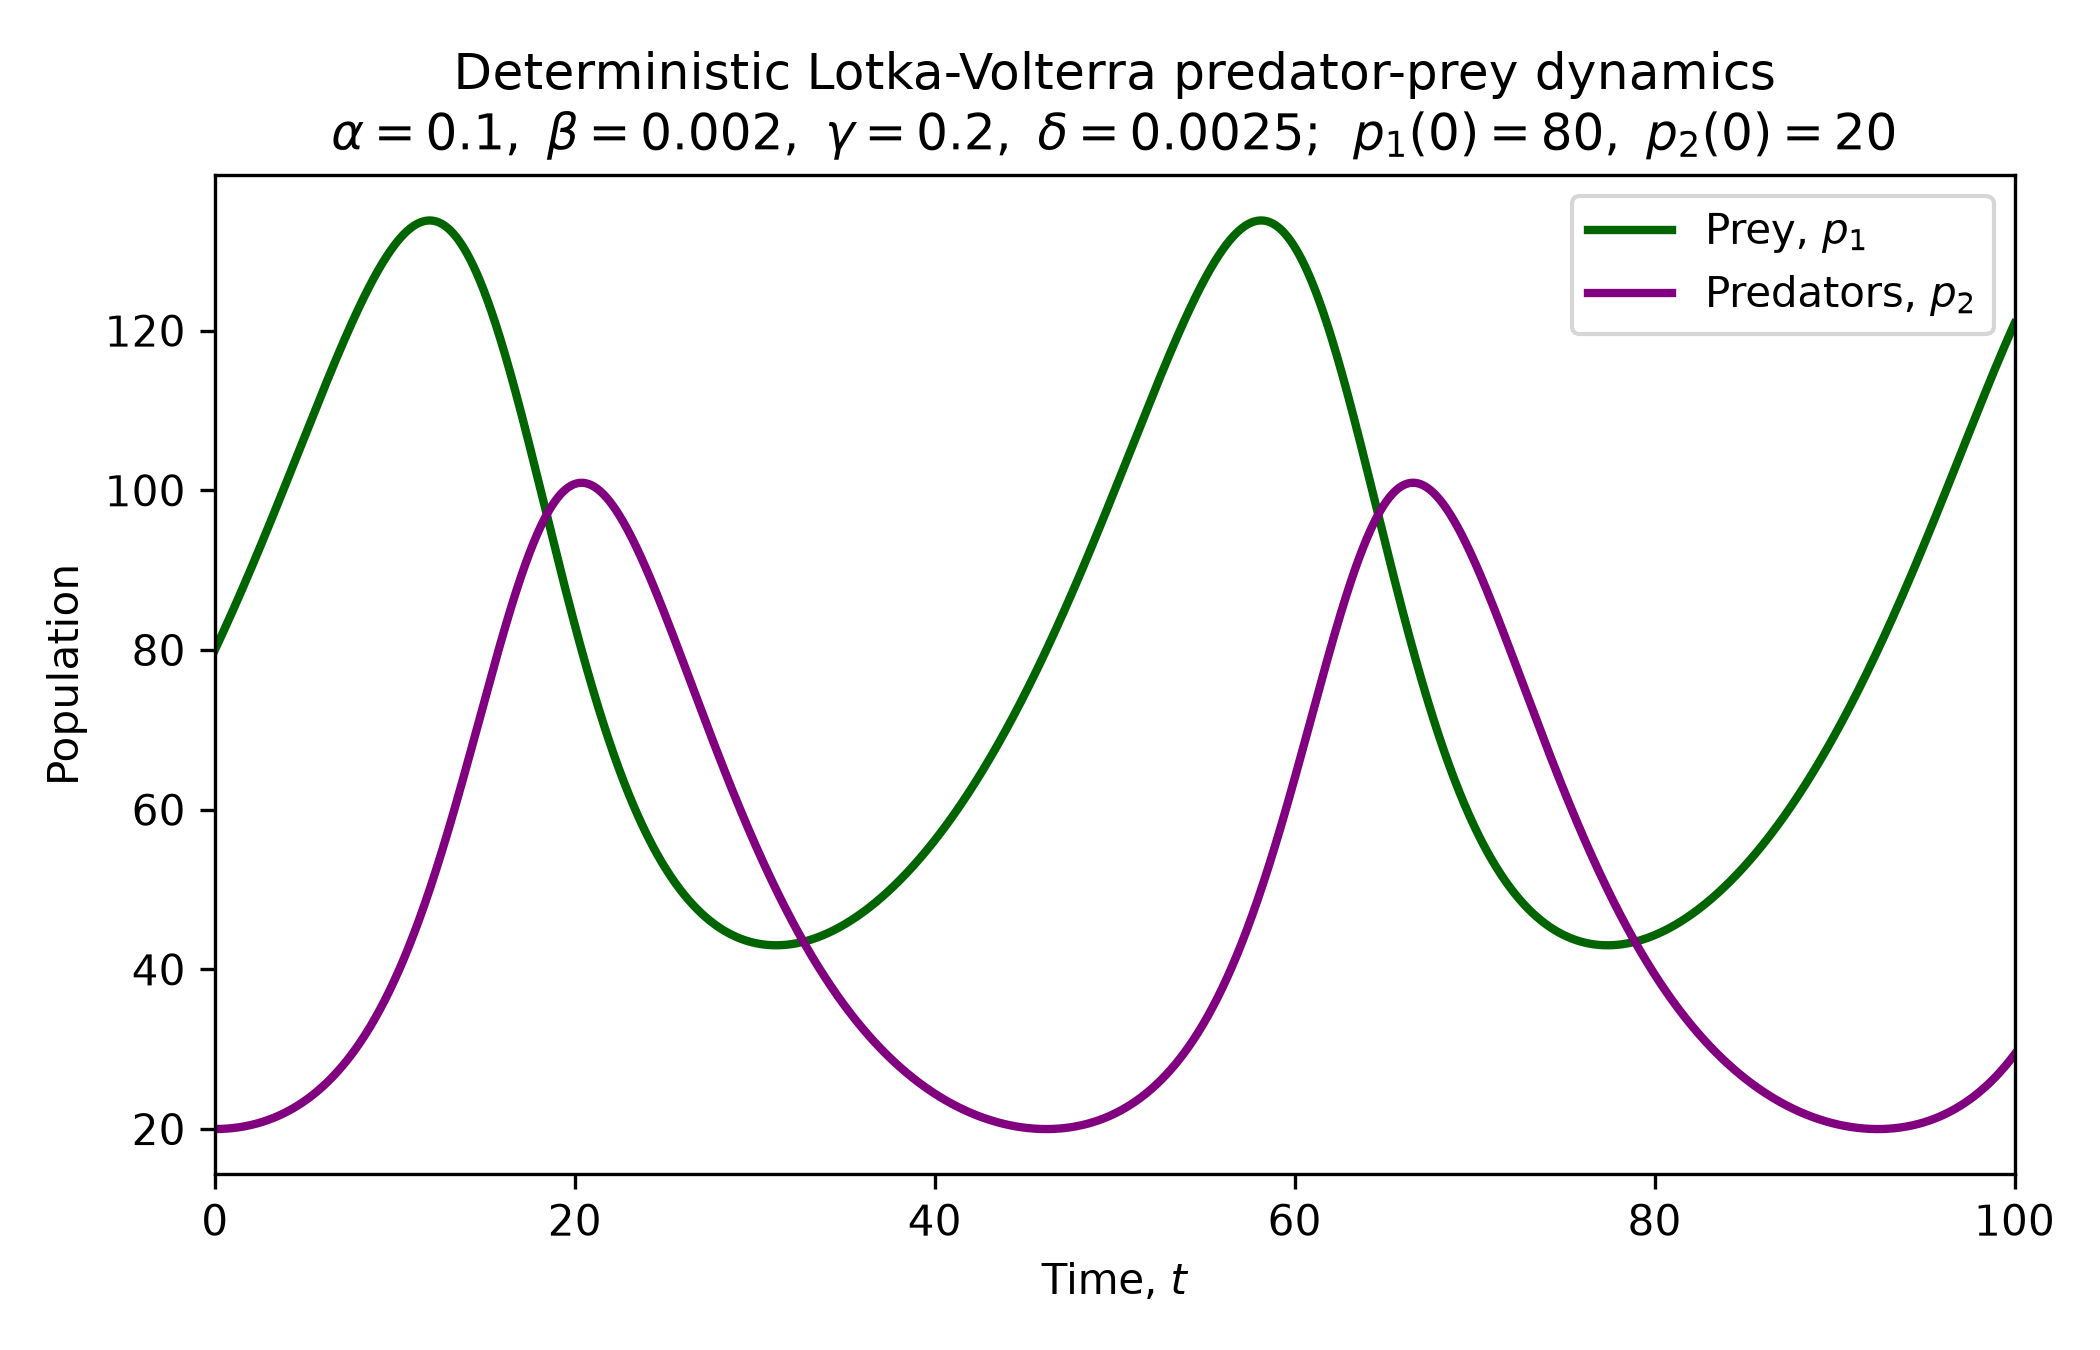
\includegraphics[width=0.85\linewidth]{figures/q1a_lotka_volterra.png}
            \caption{Deterministic Lotka-Volterra prey ($p_1$) and predator ($p_2$) populations from $t=0$ to $t=100$}
            \label{q1aLVplot}
        \end{figure}
        \item I kept the 1.a starting populations, $p_1(0)=80$ and $p_2(0)=20$, and varied only
        the rates. This gives the four outcomes in \autoref{q1bOutcomesTable}, plotted in
        \autoref{q1bOutcomesPlot}.
        \begin{table}[ht!]
            \centering
            \begin{tabular}{lcl}
                \toprule
                Outcome & $\pl \alpha, \beta, \gamma, \delta \pr$ & State by $t=100$ \\
                \midrule
                Total extinction & $\pl 0,\ 0.1,\ 0.2,\ 0.0025 \pr$ & $p_1 \to 0$, $p_2 \to 0$ \\
                Unbounded prey & $\pl 0.1,\ 0.002,\ 0.2,\ 0 \pr$ & $p_1 \to \infty$ (growing), $p_2 \to 0$ \\
                Steady coexistence & $\pl 0.1,\ 0.005,\ 0.2,\ 0.0025 \pr$ & $\pl p_1, p_2 \pr = \pl 80, 20 \pr$ for all $t$ \\
                Neutral cycles & $\pl 0.1,\ 0.002,\ 0.2,\ 0.0025 \pr$ & $p_1,p_2$ finite, bounded \\
                \bottomrule
            \end{tabular}
            \caption{Outcomes of the Lotka-Volterra model from $\pl p_1(0), p_2(0) \pr = \pl 80, 20 \pr$}
            \label{q1bOutcomesTable}
        \end{table}
        \begin{figure}[ht!]
            \centering
            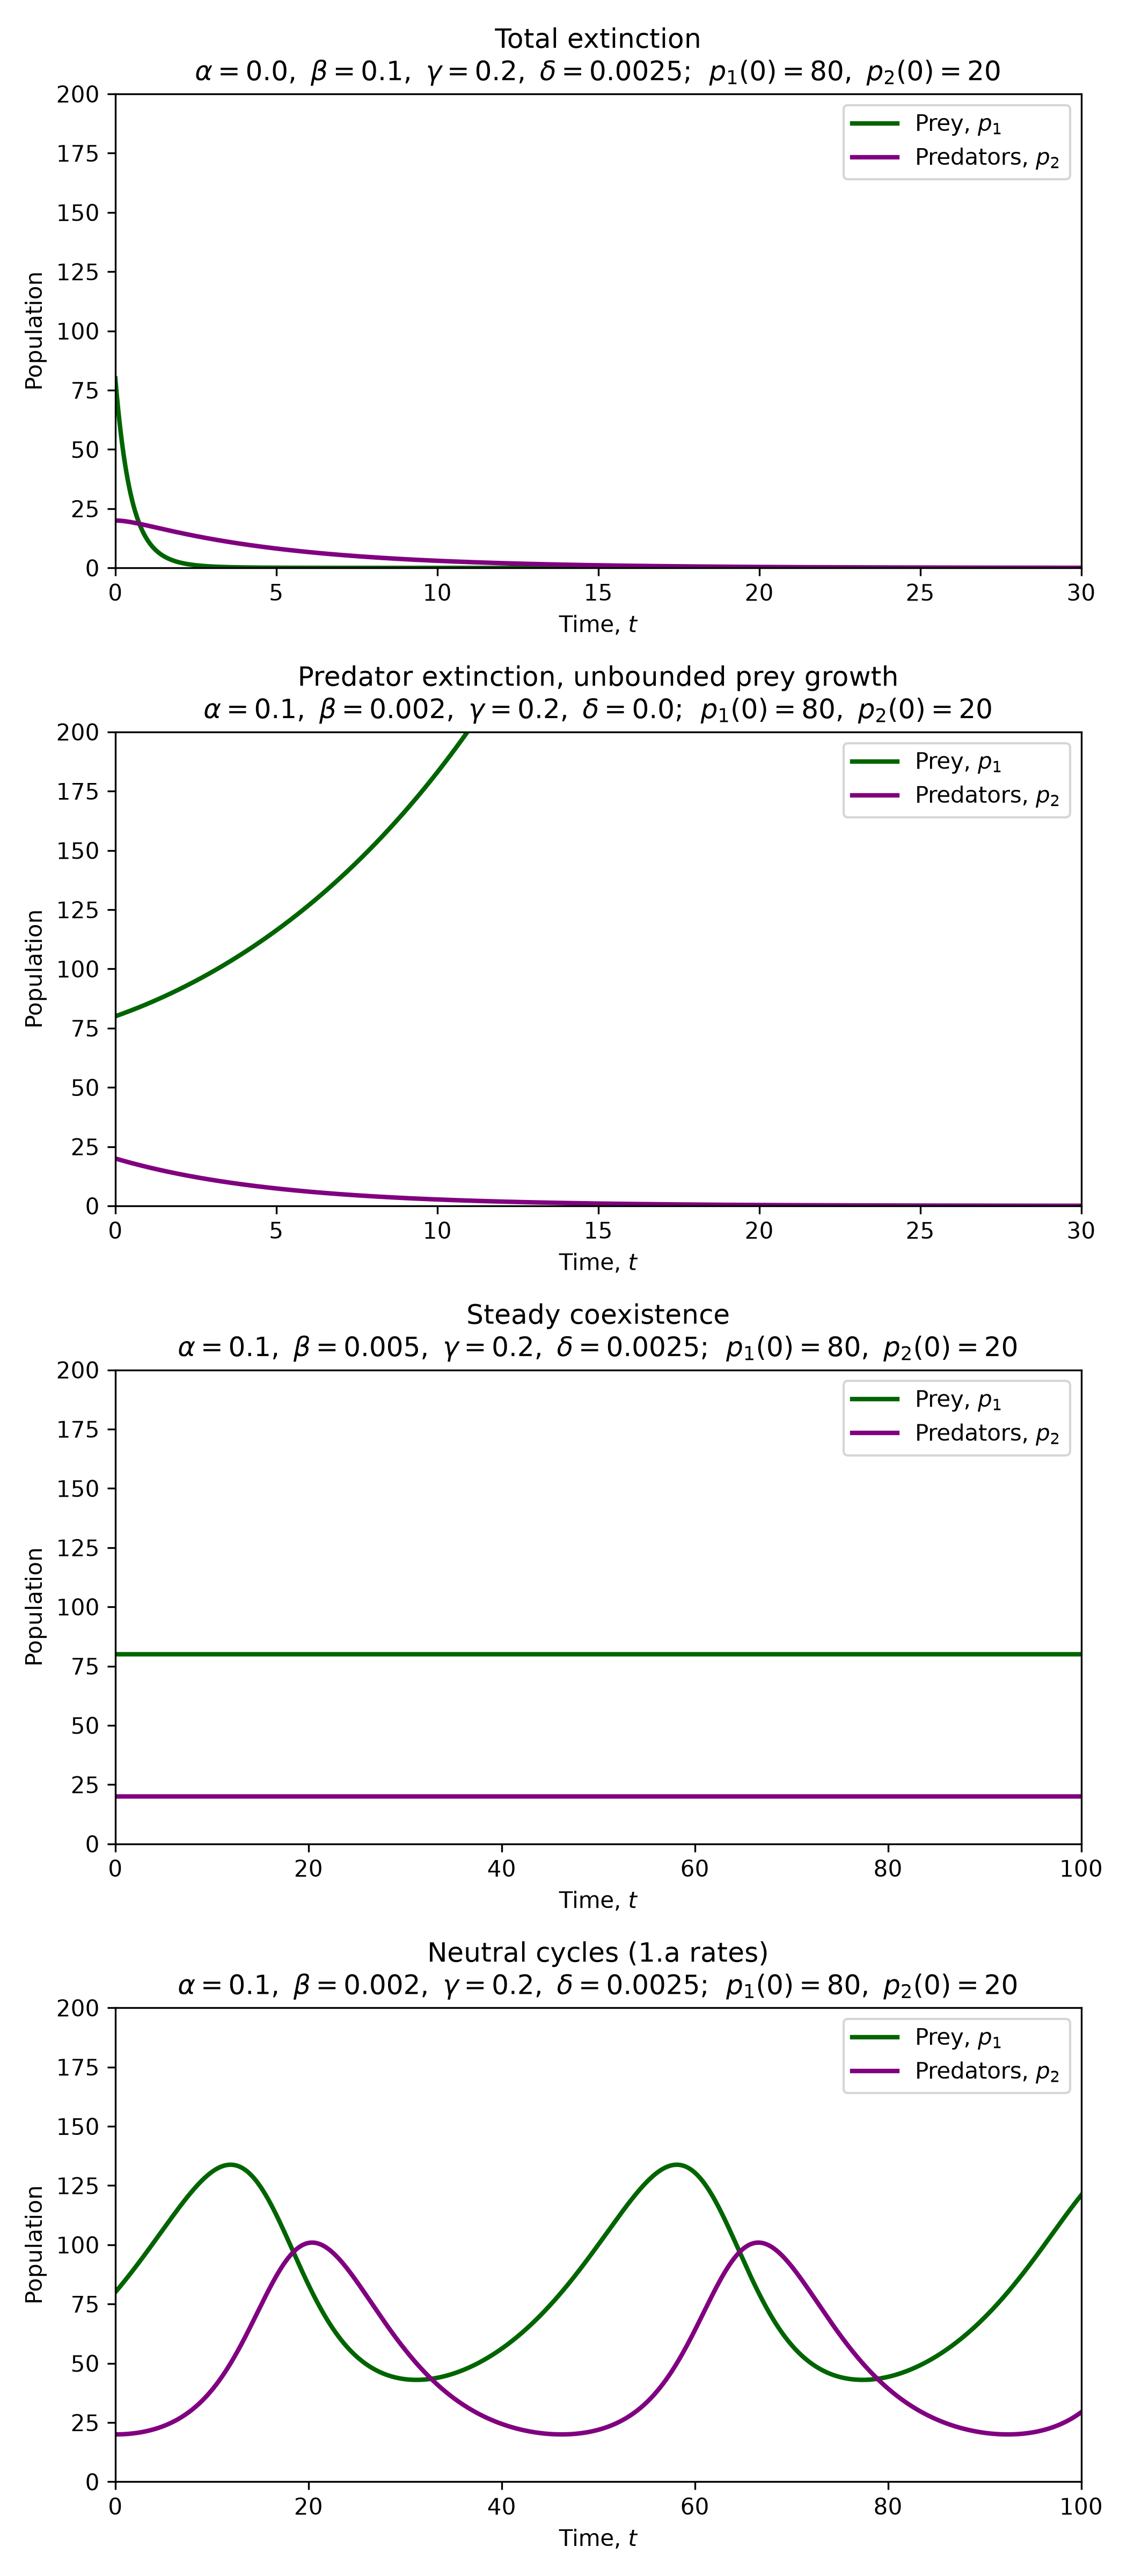
\includegraphics[height=0.8\textheight]{figures/q1b_outcomes.png}
            \caption{Population over time for each outcome in \autoref{q1bOutcomesTable}}
            \label{q1bOutcomesPlot}
        \end{figure}
        \begin{itemize}
            \item \textbf{Total extinction:} With $\alpha=0$ the prey cannot reproduce, so
            $\dfrac{dp_1}{dt} = -\beta p_1 p_2 \le 0$. With heavy predation ($\beta=0.1$), the prey fall below one
            animal extremely quickly. Then, the food term $\delta p_1$ can no longer
            balance out predator deaths. The predators then starve quickly die off by $t \approx 15$. 
            The prey actually level off at some small positive, rather than exactly $0$,
            because the predators die before eating the last fraction of a bunny. In the real world, a fraction of a bunny is no
            bunny so this is actually the $\pl 0, 0 \pr$ outcome. You can add that to a list of 
            sentences I did not think I would be typing in grad school.
            \item \textbf{Unbounded prey (predator extinction):} With $\delta=0$, eating prey never produces new
            predators, so $\dfrac{dp_2}{dt} = -\gamma p_2$ and $p_2$ falls below one animal by
            $t \approx 15$. The prey growth rate is always
            positive and will be close to purely exponential growth as the predators vanish. This is not
            a stable state, since there is no carrying capacity limit, $p_1 \to \infty$.
            \item \textbf{Steady coexistence:} With $\beta = 0.005$, $\dfrac{\alpha}{\beta} = 20$ and $\dfrac{\gamma}{\delta} = 80$,
            so the starting point is exactly the coexistence fixed point derived below in the Jacobian analysis. Both derivatives are zero
            and the populations never change.
            \item \textbf{Ongoing cycles:} The 1.a rates. Both species oscillate forever with a fixed amplitude,
            and each predator peak trails a prey peak.
        \end{itemize}

        We can use Sayama's linear stability
        analysis,\footcite{sayama2015} to prove these are the only outcomes of the model. Write the model as $\dfrac{dp_1}{dt} = F_1$ and $\dfrac{dp_2}{dt} = F_2$, with
        \begin{align*}
            F_1 &= \alpha p_1 - \beta p_1 p_2 = p_1 \pl \alpha - \beta p_2 \pr, \\
            F_2 &= \delta p_1 p_2 - \gamma p_2 = p_2 \pl \delta p_1 - \gamma \pr.
        \end{align*}
        Setting $F_1 = F_2 = 0$,
        \begin{align*}
            F_1 &= p_1 \pl \alpha - \beta p_2 \pr = 0 && \Rightarrow \quad p_1 = 0 \Or p_2 = \dfrac{\alpha}{\beta}, \\
            F_2 &= p_2 \pl \delta p_1 - \gamma \pr = 0 && \Rightarrow \quad p_2 = 0 \Or p_1 = \dfrac{\gamma}{\delta}.
        \end{align*}
        Both must hold at once. If $p_1 = 0$, then $F_2 = -\gamma p_2 = 0$ forces $p_2 = 0$. If instead
        $p_2 = \dfrac{\alpha}{\beta} \neq 0$, then $F_2 = 0$ forces $p_1 = \dfrac{\gamma}{\delta}$. This gives two fixed points,
        \begin{align*}
            \pl p_1^*, p_2^* \pr = \pl 0, 0 \pr \qquad \text{and} \qquad
            \pl p_1^*, p_2^* \pr = \pl \dfrac{\gamma}{\delta},\ \dfrac{\alpha}{\beta} \pr.
        \end{align*}
        Thus, the Jacobian is
        \begin{equation*}
            J = \begin{bmatrix}
                \dfrac{\partial F_1}{\partial p_1} & \dfrac{\partial F_1}{\partial p_2} \\[10pt]
                \dfrac{\partial F_2}{\partial p_1} & \dfrac{\partial F_2}{\partial p_2}
            \end{bmatrix}
            = \begin{bmatrix}
                \alpha - \beta p_2 & -\beta p_1 \\
                \delta p_2 & \delta p_1 - \gamma
            \end{bmatrix}.
        \end{equation*}
        \begin{itemize}
            \item At $\pl 0, 0 \pr$:
            \begin{equation*}
                J = \begin{bmatrix} \alpha & 0 \\ 0 & -\gamma \end{bmatrix},
                \qquad \lambda_1 = \alpha > 0, \quad \lambda_2 = -\gamma < 0.
            \end{equation*}
            One eigenvalue is positive and one is negative, so the origin is an unstable saddle point. 
            Along the $p_1$ axis, prey alone grow like $e^{\alpha t}$. Along the $p_2$ axis, predators alone die
            like $e^{-\gamma t}$. A trajectory that starts with both populations positive can never reaches the
            origin.
            \item At $\pl \dfrac{\gamma}{\delta},\ \dfrac{\alpha}{\beta} \pr$:
            \begin{equation*}
                J = \begin{bmatrix} 0 & -\dfrac{\beta\gamma}{\delta} \\[4pt] \dfrac{\alpha\delta}{\beta} & 0 \end{bmatrix},
                \qquad \det\pl J - \lambda I \pr = \lambda^2 + \alpha\gamma = 0
                \quad \Rightarrow \quad \lambda = \pm i\sqrt{\alpha\gamma}.
            \end{equation*}
            The eigenvalues are purely imaginary, so the linearization is a center. Because
            $\mathrm{Re}\,\lambda = 0$, linearization alone cannot tell us whether the full nonlinear system expands, contracts, or cycles. 
        \end{itemize}
        So, to settle the center case, we will use a Lyapunov function. The quantity
        \begin{equation*}
            V\pl p_1, p_2 \pr = \delta p_1 - \gamma \ln p_1 + \beta p_2 - \alpha \ln p_2
        \end{equation*}
        is conserved along every trajectory:
        \begin{align*}
            \dfrac{dV}{dt} &= \pl \delta - \dfrac{\gamma}{p_1} \pr \dfrac{dp_1}{dt} + \pl \beta - \dfrac{\alpha}{p_2} \pr \dfrac{dp_2}{dt} \\
            &= \pl \delta - \dfrac{\gamma}{p_1} \pr p_1 \pl \alpha - \beta p_2 \pr + \pl \beta - \dfrac{\alpha}{p_2} \pr p_2 \pl \delta p_1 - \gamma \pr \\
            &= \pl \delta p_1 - \gamma \pr \pl \alpha - \beta p_2 \pr + \pl \beta p_2 - \alpha \pr \pl \delta p_1 - \gamma \pr = 0.
        \end{align*}
        $V$ has its minimum at $\pl \dfrac{\gamma}{\delta},\ \dfrac{\alpha}{\beta} \pr$, and it goes to infinity whenever either
        population goes to $0$ or to $\infty$. So every trajectory stays on one closed level curve of $V$ for all timesteps. Thus, we have two conclusions:
        \begin{enumerate}
            \item The coexistence scenario is Lyapunov stable but not asymptotically stable, so it will orbit that
            start point, staying near, but never converging to it. It is neutrally stable.
            \item Orbits can neither reach the axes nor escape to infinity.
        \end{enumerate}
        Thus, for $\alpha, \beta, \gamma, \delta > 0$ and $p_1(0), p_2(0) > 0$, the only possible outcomes are
        steady coexistence (starting exactly at the fixed point) and neutral cycles (starting anywhere else). The
        model has no attracting sink at all. Extinction or explosion requires zeroing a rate ($\alpha = 0$
        or $\delta = 0$, as above) or starting with a population of zero: $p_2(0) = 0$ gives
        $p_1 = p_1(0)e^{\alpha t}$, and $p_1(0) = 0$ gives $p_2 = p_2(0)e^{-\gamma t}$.

        Finally, with the 1.a rates and
        $\pl p_1(0), p_2(0) \pr = \pl 50, 50 \pr$, See \autoref{q1bVariedStart}, $p_2(0) = \dfrac{\alpha}{\beta} = 50$ makes
        $\dfrac{dp_1}{dt} = 0$ at $t=0$, so the run starts at the bottom of a prey cycle. 
        \autoref{q1bPhasePortrait} puts all 5 of these these phase patterns together in a single plane. The orbits are nested closed loops
        around the center at $\pl 80, 50 \pr$, each a level curve of $V$, travelled counterclockwise, with the saddle at the origin.
        \begin{figure}[ht!]
            \centering
            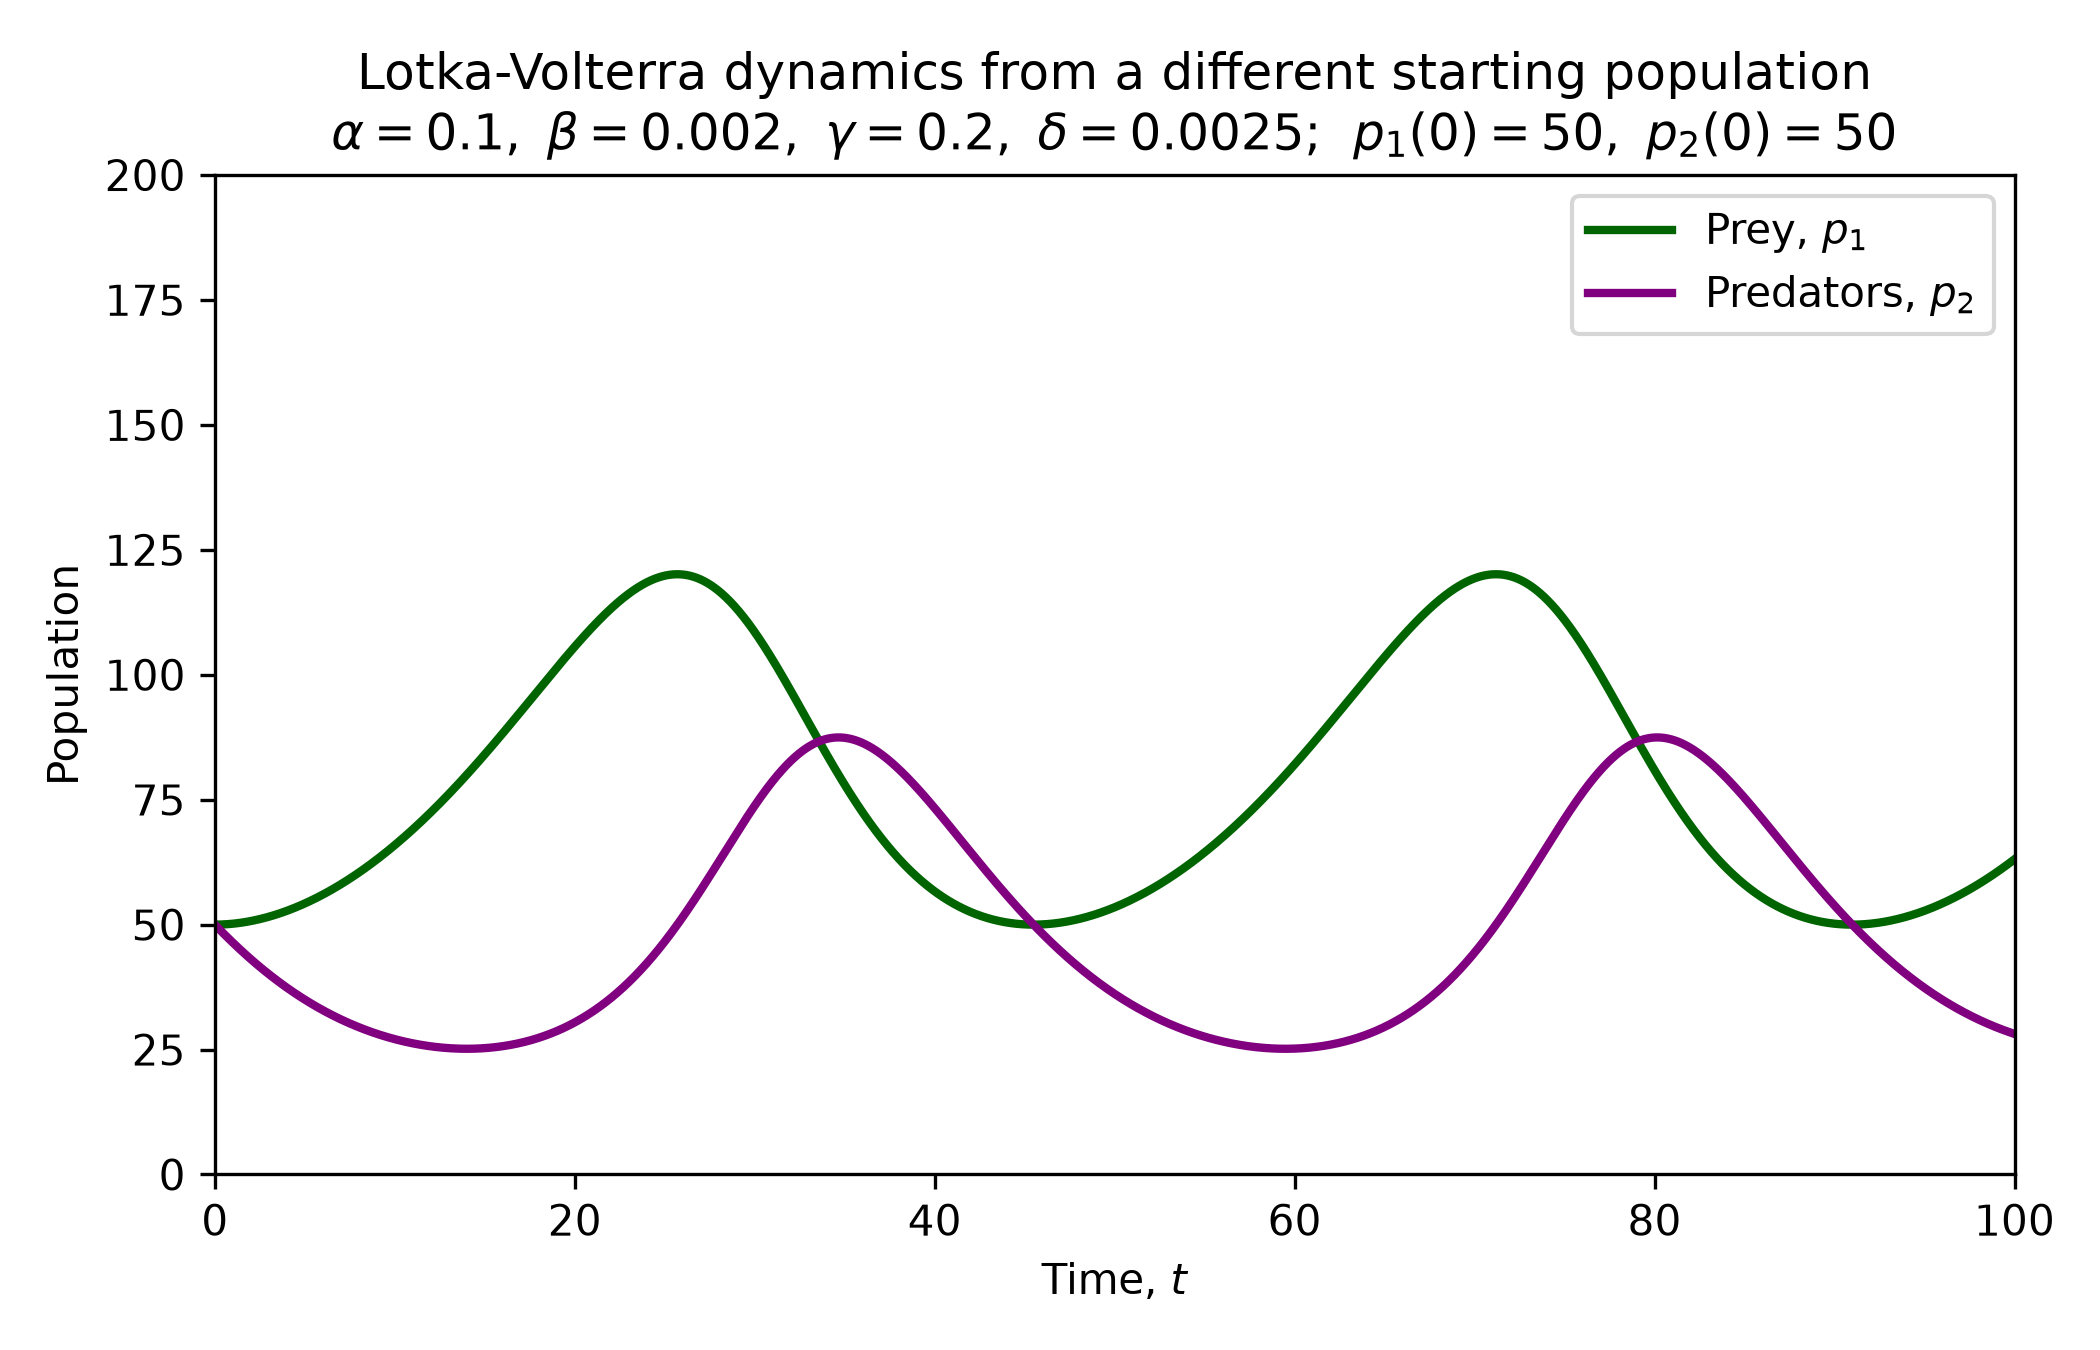
\includegraphics[width=0.85\linewidth]{figures/q1b_varied_start.png}
            \caption{Lotka-Volterra populations from $\pl p_1(0), p_2(0) \pr = \pl 50, 50 \pr$ with the 1.a rates}
            \label{q1bVariedStart}
        \end{figure}
        \begin{figure}[ht!]
            \centering
            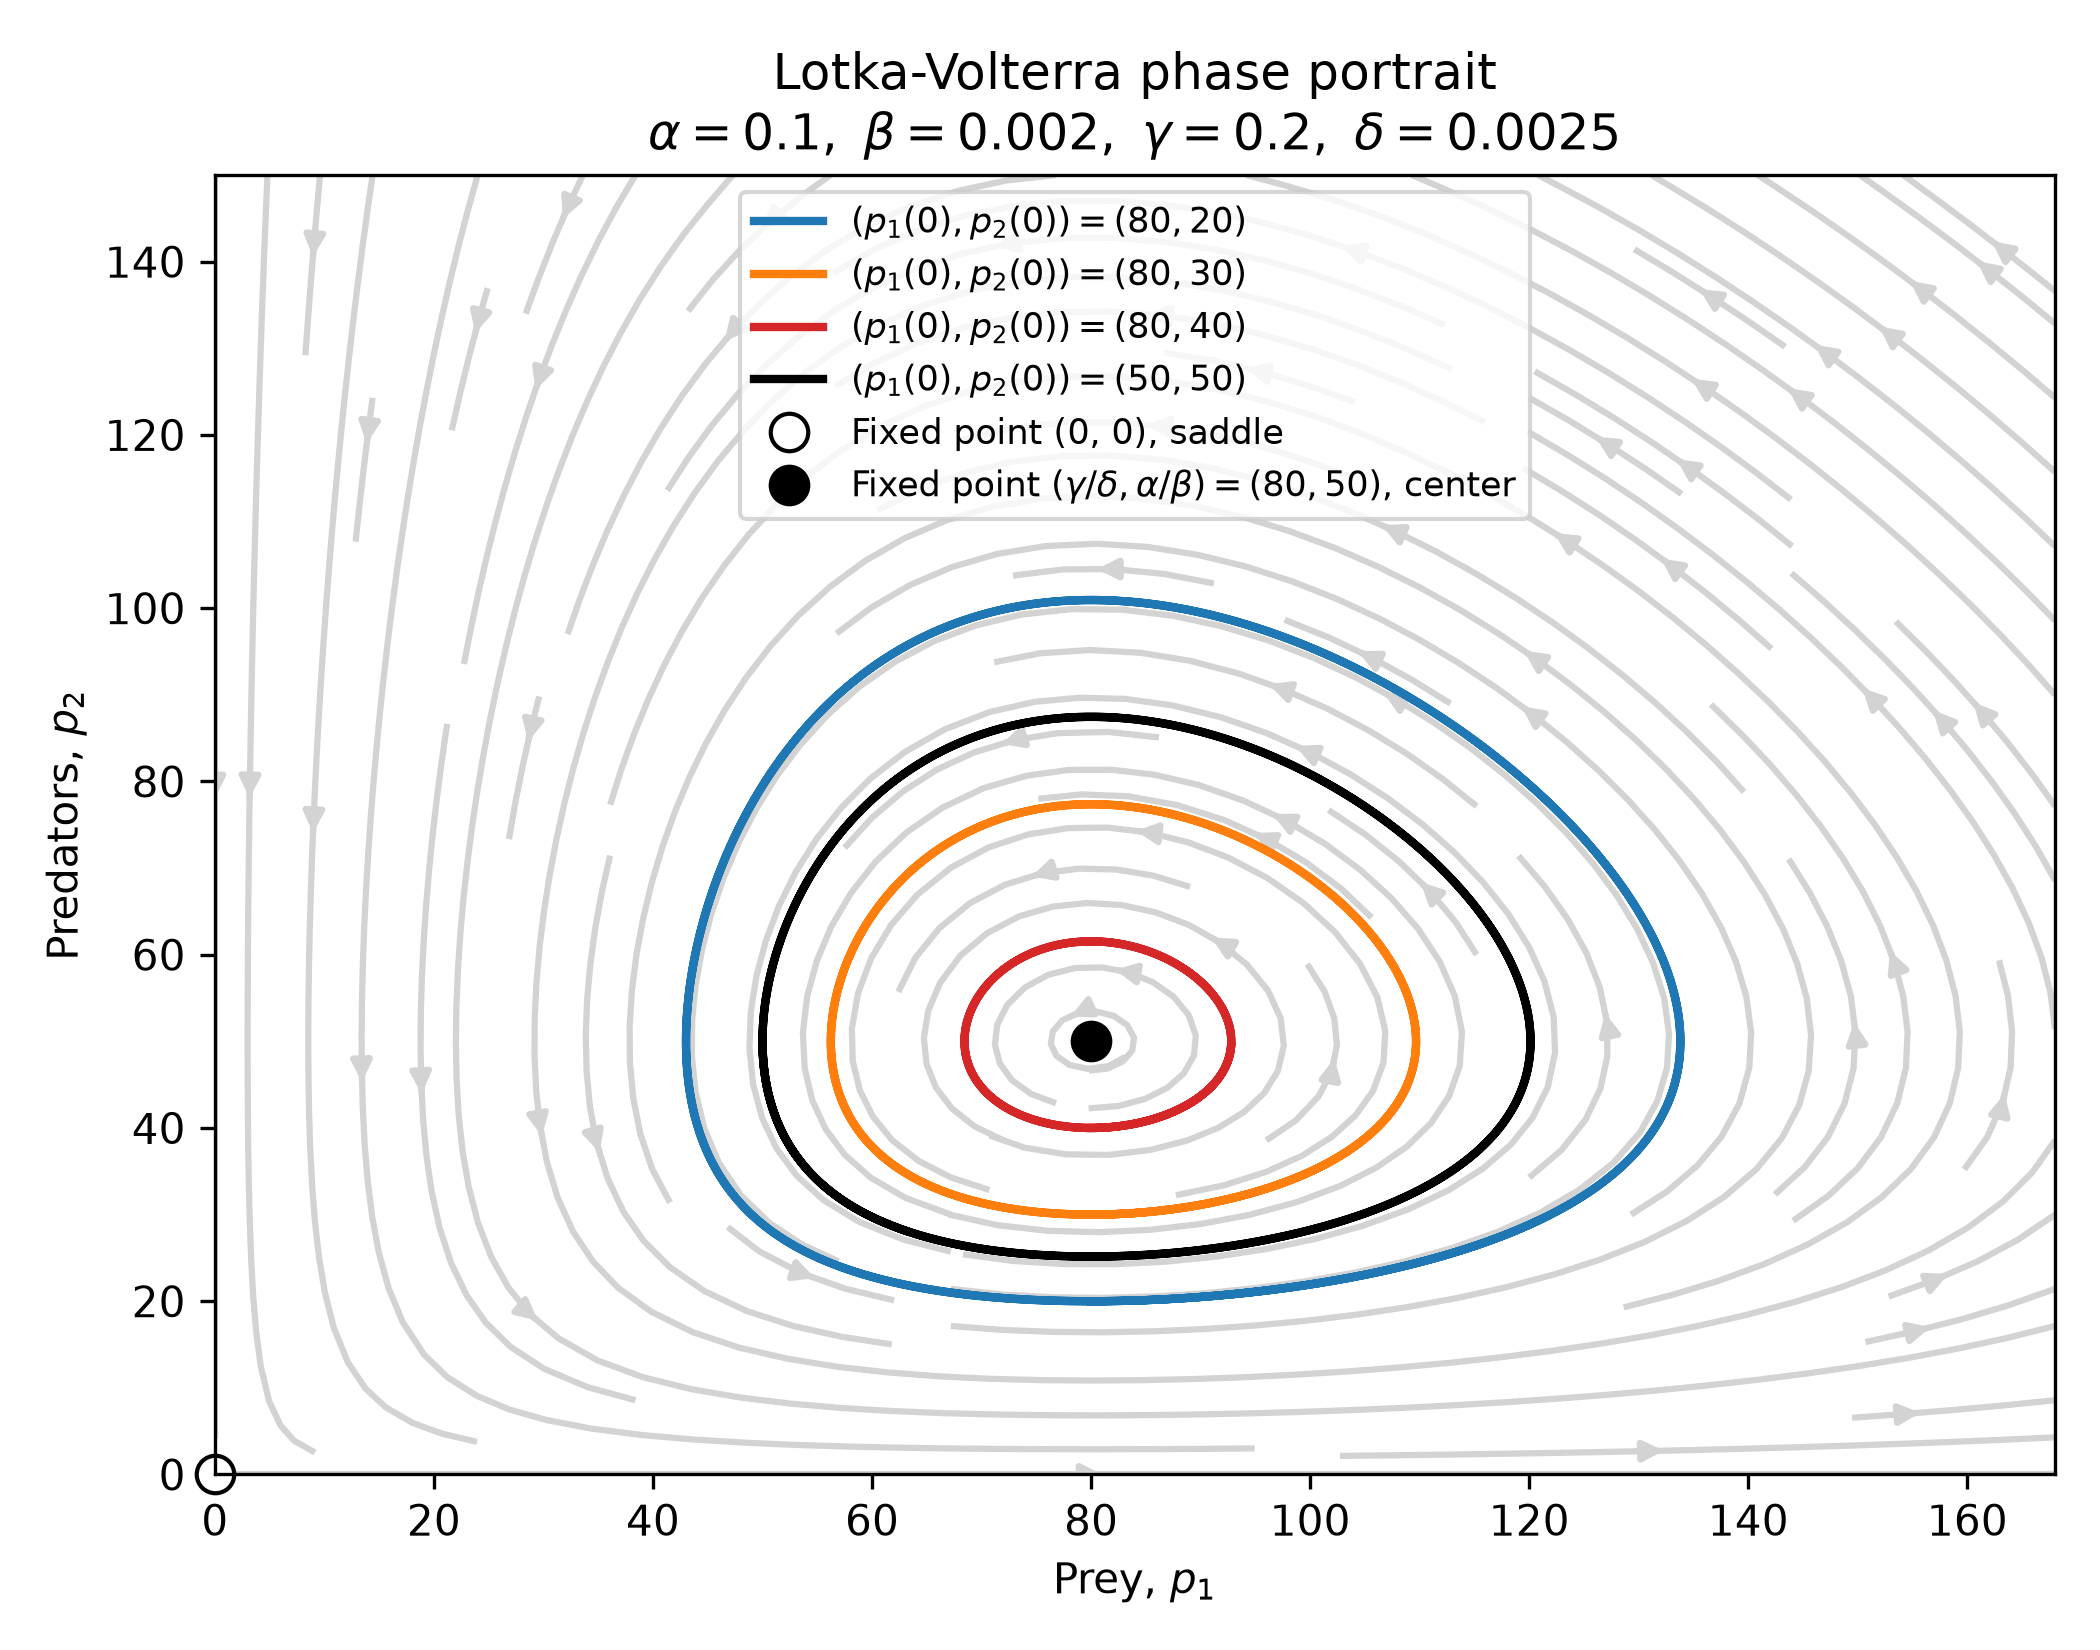
\includegraphics[width=0.85\linewidth]{figures/q1b_phase_portrait.png}
            \caption{Phase portrait of L-V model with 1.a rates}
            \label{q1bPhasePortrait}
        \end{figure}
        \item To see why L-V cycles, we can look back at the two core drivers from 1.b above.
        First, the model has two independent populations that rely on one another, since predators 
        eat the prey, which suppresses the prey pop., which suppresses the predator pop. Second, this
        rotation (in phase space) of predator peak following prey peak is also always conserved. The
        Lyapunov function above shows $V$ is never allowing the orbits to crash or expand. Thus, 
        the rotation lasts forever and we see the cycles in the population plots. 

        SIS model looks similar, but lacks this long term rotating stability. If we look at the
        rate equations 
        \begin{align*}
            \dfrac{dS}{dt} &= -\beta \dfrac{SI}{N} + \mu I, \\
            \dfrac{dI}{dt} &= \beta \dfrac{SI}{N} - \mu I.
        \end{align*}
        we can see that the $\beta \dfrac{SI}{N}$ infection term plays the role of predator,
        while recovery back to the S compartment is analagous to predator death. The core 
        difference is that $S+I=N$ is fixed, whereas in L-V total population is not (no
        carrying capacity constraints). Substituting $S = N - I$,
        \begin{align*}
            \dfrac{dI}{dt} &= \beta \dfrac{SI}{N} - \mu I = \beta I\pl\dfrac{N-1}{N}\pr-\mu I=\beta I \pl 1 - \dfrac{I}{N} \pr - \mu I,
        \end{align*}
        we can see that it is an equation on the single variable $I$. If $\dfrac{dI}{dt}$ depends only on $I$,
        it can only move steadily towards a fixed point, because to reverse direction would requiring
        going through $\dfrac{dI}{dt}=0$, which is a fixed point, which would halt the process. 
        Thinking in terms of the Jacobian, the Jacobian of a one-variable model is a single number, so 
        the eigenvalue is always real and cannot generate the imaginary pair required for ongoing rotation. 
        
        SIR does not produce cycling behavior either. 
        \begin{align*}
            \dfrac{dS}{dt} &= -\beta \dfrac{SI}{N}, \\
            \dfrac{dI}{dt} &= \beta \dfrac{SI}{N} - \mu I, \\
            \dfrac{dR}{dt} &= \mu I
        \end{align*}
        With $N$ fixed it reduces to two variables, so it
        could cycle on dimension based on that alone, but
        \begin{align*}
            \dfrac{dS}{dt} = -\beta \dfrac{SI}{N} \le 0, \quad \text{because }\beta,S,I,N>0
        \end{align*}
        so $S$ only ever decreases. A closed loop would need $S$ to return to its starting value, which 
        cannot happen so we get a single epidemic wave in which $I$ rises and then falls to $0$. 
        
        SIRS, however,  adds a return feature ($R \to S$), which refills the susceptibles much like the prey birth term $\alpha p_1$.
        \begin{align*}
            \dfrac{dS}{dt} &= -\beta \dfrac{SI}{N} + \omega R, \\
            \dfrac{dI}{dt} &= \beta \dfrac{SI}{N} - \mu I, \\
            \dfrac{dR}{dt} &= \mu I - \omega R, \qquad \text{($\omega$: rate of return to $S$)}
        \end{align*}
        This allows oscillations, but they are dampened. Intuitively, the total population is capped at
        $S + I + R = N$, so a burst of infections uses up the susceptibles it requires, and each compartment
        drains in proportion to its own size ($\mu I$ out of $I$, $\omega R$ out of $R$). Each overshoot is
        then followed by a smaller one, like a damped spring, and the system settles to a steady state (clearly visible in
        the SIRS plots from class). In L-V
        nothing caps the total population and $V$ is conserved, so nothing is lost and the swings never shrink.
        So SIRS can oscillate, but it does not sustain cycles. \autoref{q1cSIRSplot} shows this, after the
        first large wave, each swing is smaller than the last, and all three compartments flatten out.
        \begin{figure}[ht!]
            \centering
            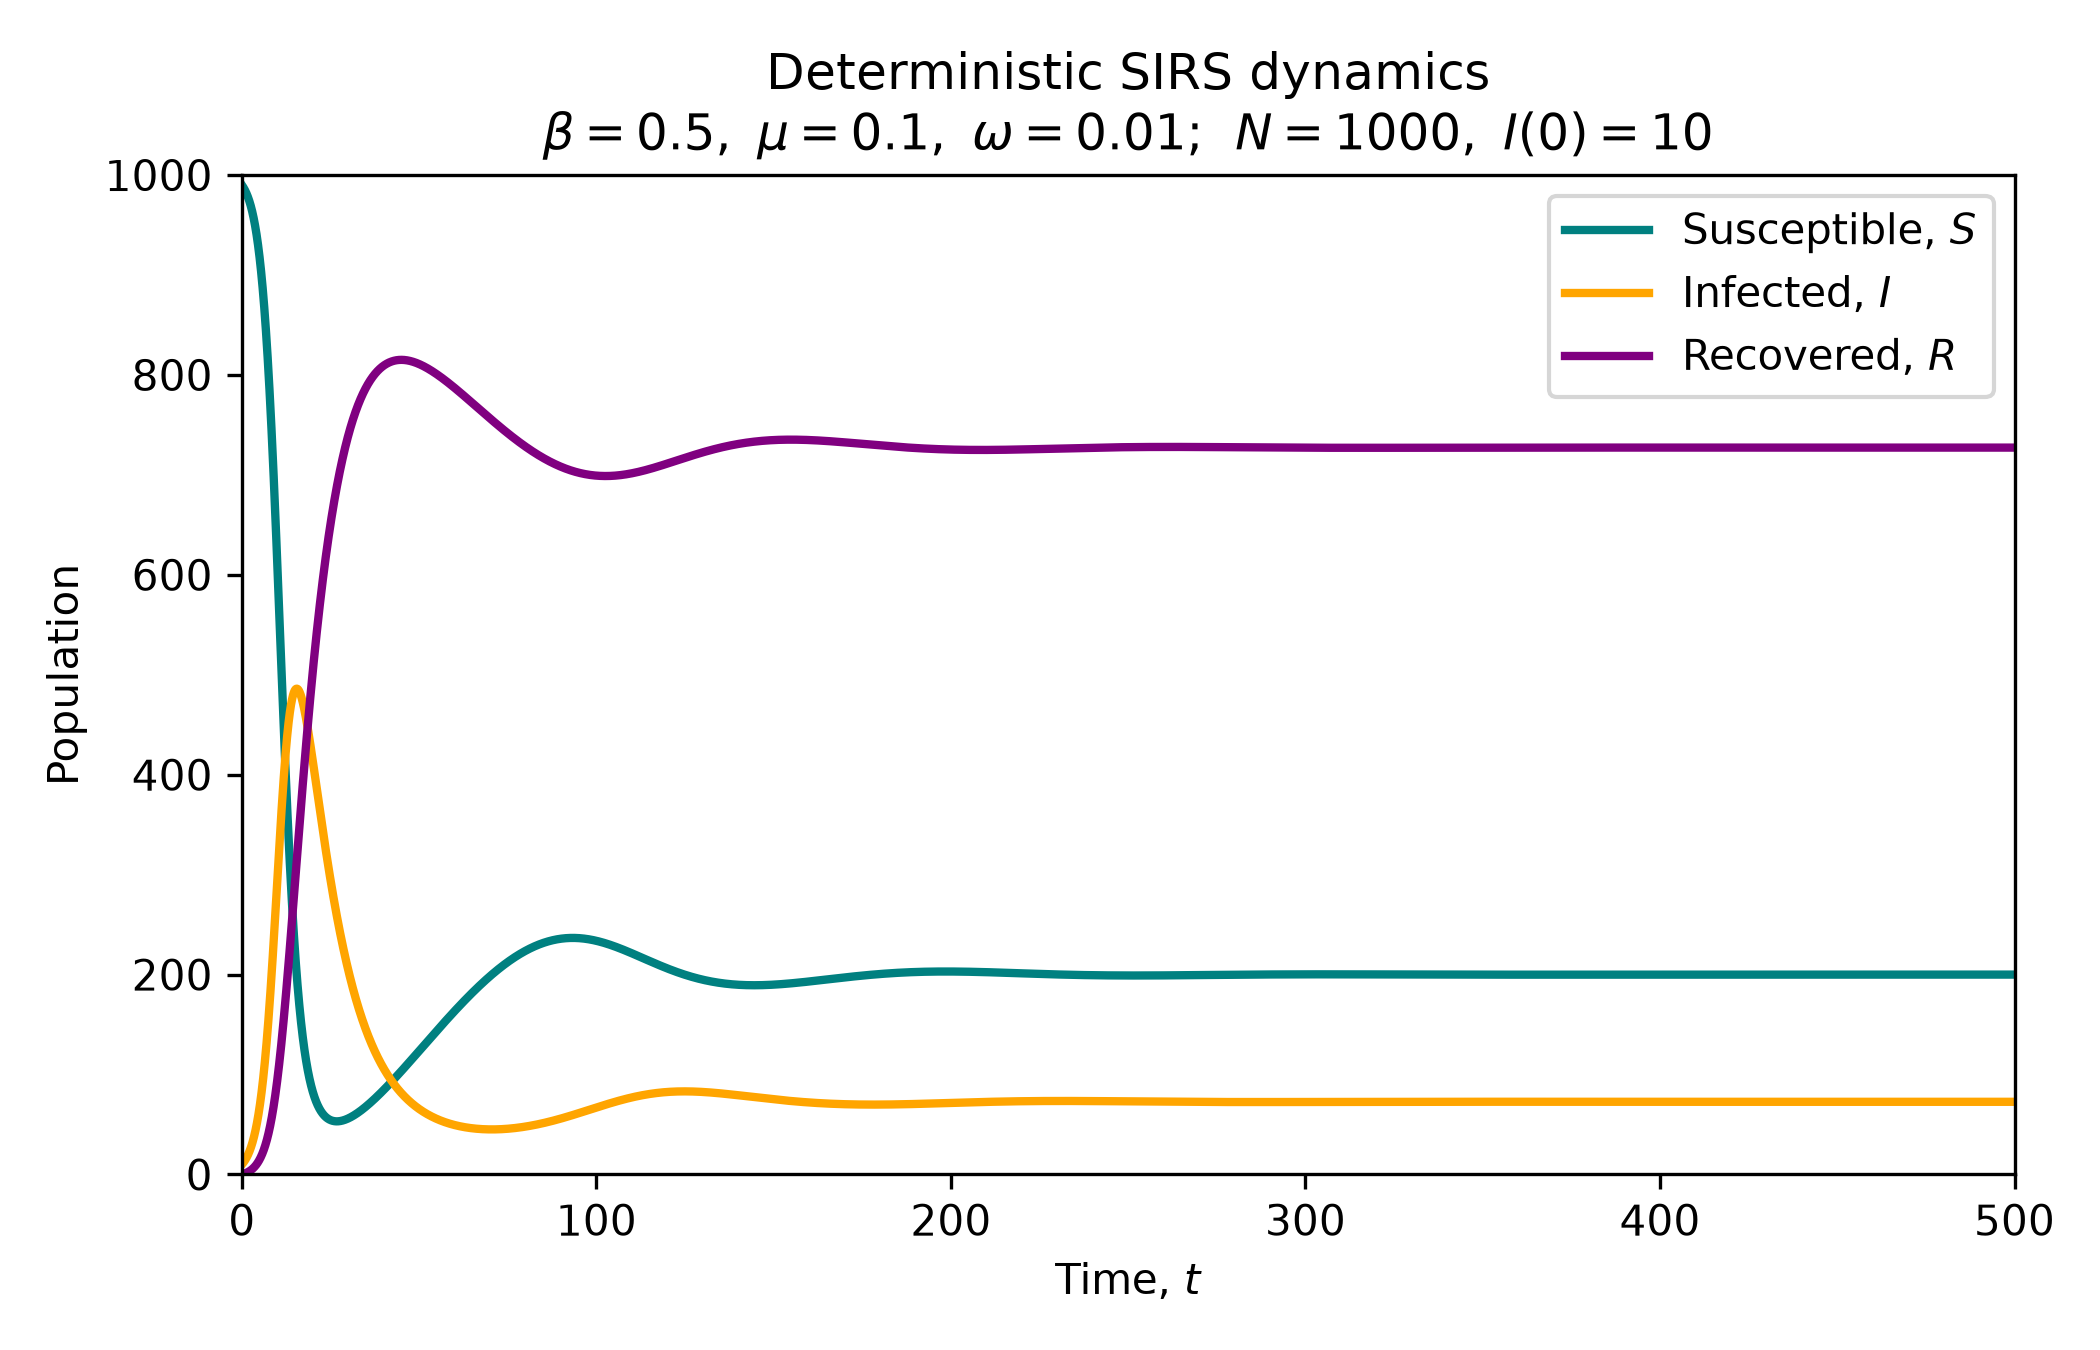
\includegraphics[width=0.85\linewidth]{figures/q1c_sirs.png}
            \caption{Deterministic SIRS populations showing damped oscillations that settle to a steady state}
            \label{q1cSIRSplot}
        \end{figure}

        This is far from a proper proof, but to be honest, I think I've already spent
        way too much time on this question so far, so I'm doing a little hand-waving
        here at the end and appealing to intuition, sorry.

        \textbf{Core takeway:}\\
        Sustained cycles need three things: a second independent population, feedback of opposite signs
        between the two, and no damping. SIS fails the first, SIR fails the second because nothing refills
        $S$, and SIRS fails the third.
        \clearpage
    \end{enumerate}
\end{enumerate}
\end{solution}

\begin{problem}{2 (40 points)}

    We will now adapt Lotke-Volterra to a network setting. We will take a graph $G$ as an argument, and assign ratio $x$ nodes to start as prey, ratio $y$ nodes to start as predators, and all other nodes to begin as ``empty." For example, here is our favorite Karate Club graph with blue prey (0.4), red predators (0.1), and gray empty vertices:

    \begin{center}
    \begin{tikzpicture}
        \SetDistanceScale{2.5}
        \SetVertexStyle{LineOpacity=0}
        \Vertices[shape=circle,NoLabel=True,size=0.25]{givenfiles_CNET5051_Assignment3_2026/kc_vert.csv}
        \Edges[]{givenfiles_CNET5051_Assignment3_2026/kc_edges.csv}
    \end{tikzpicture}
    \end{center}

    At each timestep, each prey animal may, with probability $\alpha$, ``reproduce'' by turning a randomly-chosen empty neighboring vertex into a prey vertex. Each prey animal may be eaten by each neighboring predator (and replaced with an empty vertex) with probability $\beta$. If the predator eats a prey animal there is a $\delta$ chance of that vertex becoming another predator vertex instead of empty. Finally, each predator may die and become an empty cell with probability $\gamma$.
    
    \begin{enumerate}[label=(\alph*)]
        \item Implement the simulation (20 points).
        
        Implement the above simulation in Python, creating a function with the signature:

        \begin{lstlisting}[language=Python,numbers=none]
def graphLotkeVolterra(G, x, y, alpha, beta, gamma, delta, T)
        \end{lstlisting}

        This simulation runs for T time steps, and returns a list of the simulation state at each time step. You may return a list of networkx graphs, or a list of tuples representing predator and prey populations. Here is one example of species progression over time in the Karate club graph:

        \begin{center}
            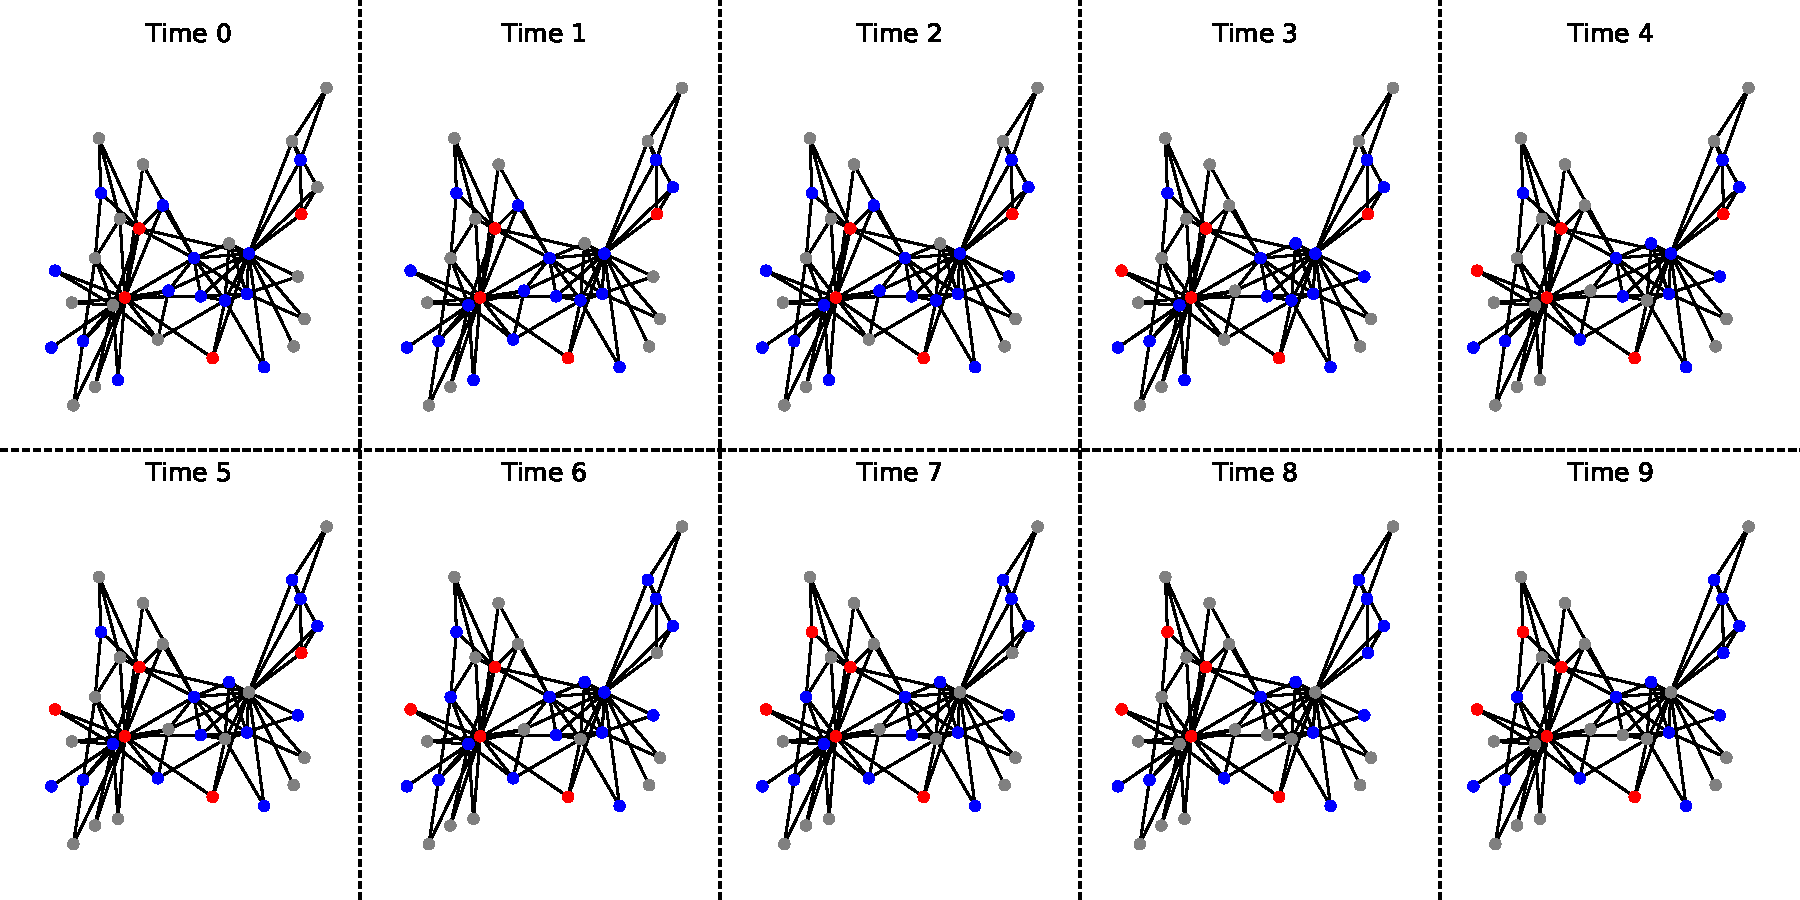
\includegraphics[width=0.9\linewidth]{givenfiles_CNET5051_Assignment3_2026/kc_progression.pdf}
        \end{center}

        If you need to adjust starting populations or your $\alpha, \beta, \gamma, \delta$ parameters to produce interesting results, do so. For example, if you find that all the predators quickly die without reproducing, you may need to increase $\beta$ or $\gamma$ or decrease $\delta$ a little.
        
        You do not need to produce a plot like the one above, but it may help your debugging.

        \item Influence of Network Structure on Population (10 points).

        Create the following graphs: 2d-grid, Erd\"{o}s-R\'{e}nyi, Barabasi, and Watts-Strogatz small-world using the following parameters:

        \begin{lstlisting}[language=python,numbers=none]
G1 = nx.grid_2d_graph(100, 100)
G2 = nx.gnp_random_graph(1000, 0.05)
G3 = nx.barabasi_albert_graph(1000, 2)
G4 = nx.watts_strogatz_graph(1000, 2, 0.05)
        \end{lstlisting}
        
        Run your simulation on each for at least 100 time steps. For each simulation, produce a plot of predator and prey populations over time.

        \item Discussion (10 points).

        What effect does network topology have on predator-prey dynamics? Are some topologies more advantageous for one species or the other, are some more favorable to stable equilibrium? Why?

        
    \end{enumerate}
\end{problem}

\begin{solution}
\begin{enumerate}
    \item [] \begin{enumerate}
        \item See \texttt{.ipynb} for code. \texttt{graphLotkeVolterra(G, x, y, alpha, beta, gamma, delta, T, seed)}
        returns a list of $T+1$ tuples (prey, predators), one for each time step including $t=0$. I added an
        optional \texttt{seed} so any run can be reproduced exactly. At the start, $\mathrm{round}\pl xN \pr$ random
        nodes become prey, $\mathrm{round}\pl yN \pr$ become predators, and the rest are empty.

        Each time step is a synchronous update: every decision is made from the state at time $t$ and the changes
        are applied all at once, the same idea as the status/next status approach in the class 13 epidemic code.
        At each step:
        \begin{itemize}
            \item each prey, with probability $\alpha$, picks a random empty neighbor and fills it with a new prey,
            \item each neighboring predator gets its own chance $\beta$ to eat a given prey, so a prey with $k_Z$
            predator neighbors is eaten with probability
            \begin{align*}
                P\pl \text{eaten} \pr = 1 - \pl 1 - \beta \pr^{k_Z},
            \end{align*}
            and the eaten prey's vertex becomes a predator with probability $\delta$ (otherwise it becomes empty),
            \item each predator dies with probability $\gamma$.
        \end{itemize}
        The question leaves a few conflicts open, so I made these choices (commented in the code):
        \begin{itemize}
            \item If two prey pick the same empty node, the lower-indexed prey gets it and the higher-indexed prey
            loses its turn.
            \item Birth before death: a prey that is eaten this step may still reproduce.
            \item Meal before death: a predator that dies this step may still eat.
        \end{itemize}
        Two separate functions handle plotting. One draws 10 snapshots of the network ($t = 1, \dots, 5$, then 5
        times spread over the rest of the run), and the other plots the three populations over time as a percent of
        the $N$ nodes. \autoref{q2aSnapshots} and \autoref{q2aPopulations} show a run on the karate club graph with
        $x = 0.4$ and $y = 0.1$ as in the example above, and $\pl \alpha, \beta, \gamma, \delta \pr = \pl 0.5,\ 0.1,\ 0.1,\ 0.5 \pr$.
        The prey first fill most of the empty nodes, the predators then catch up, and after that the populations
        trade off noisily. With only 34 nodes, the details of a run depend a lot on the seed.
        \begin{figure}[ht!]
            \centering
            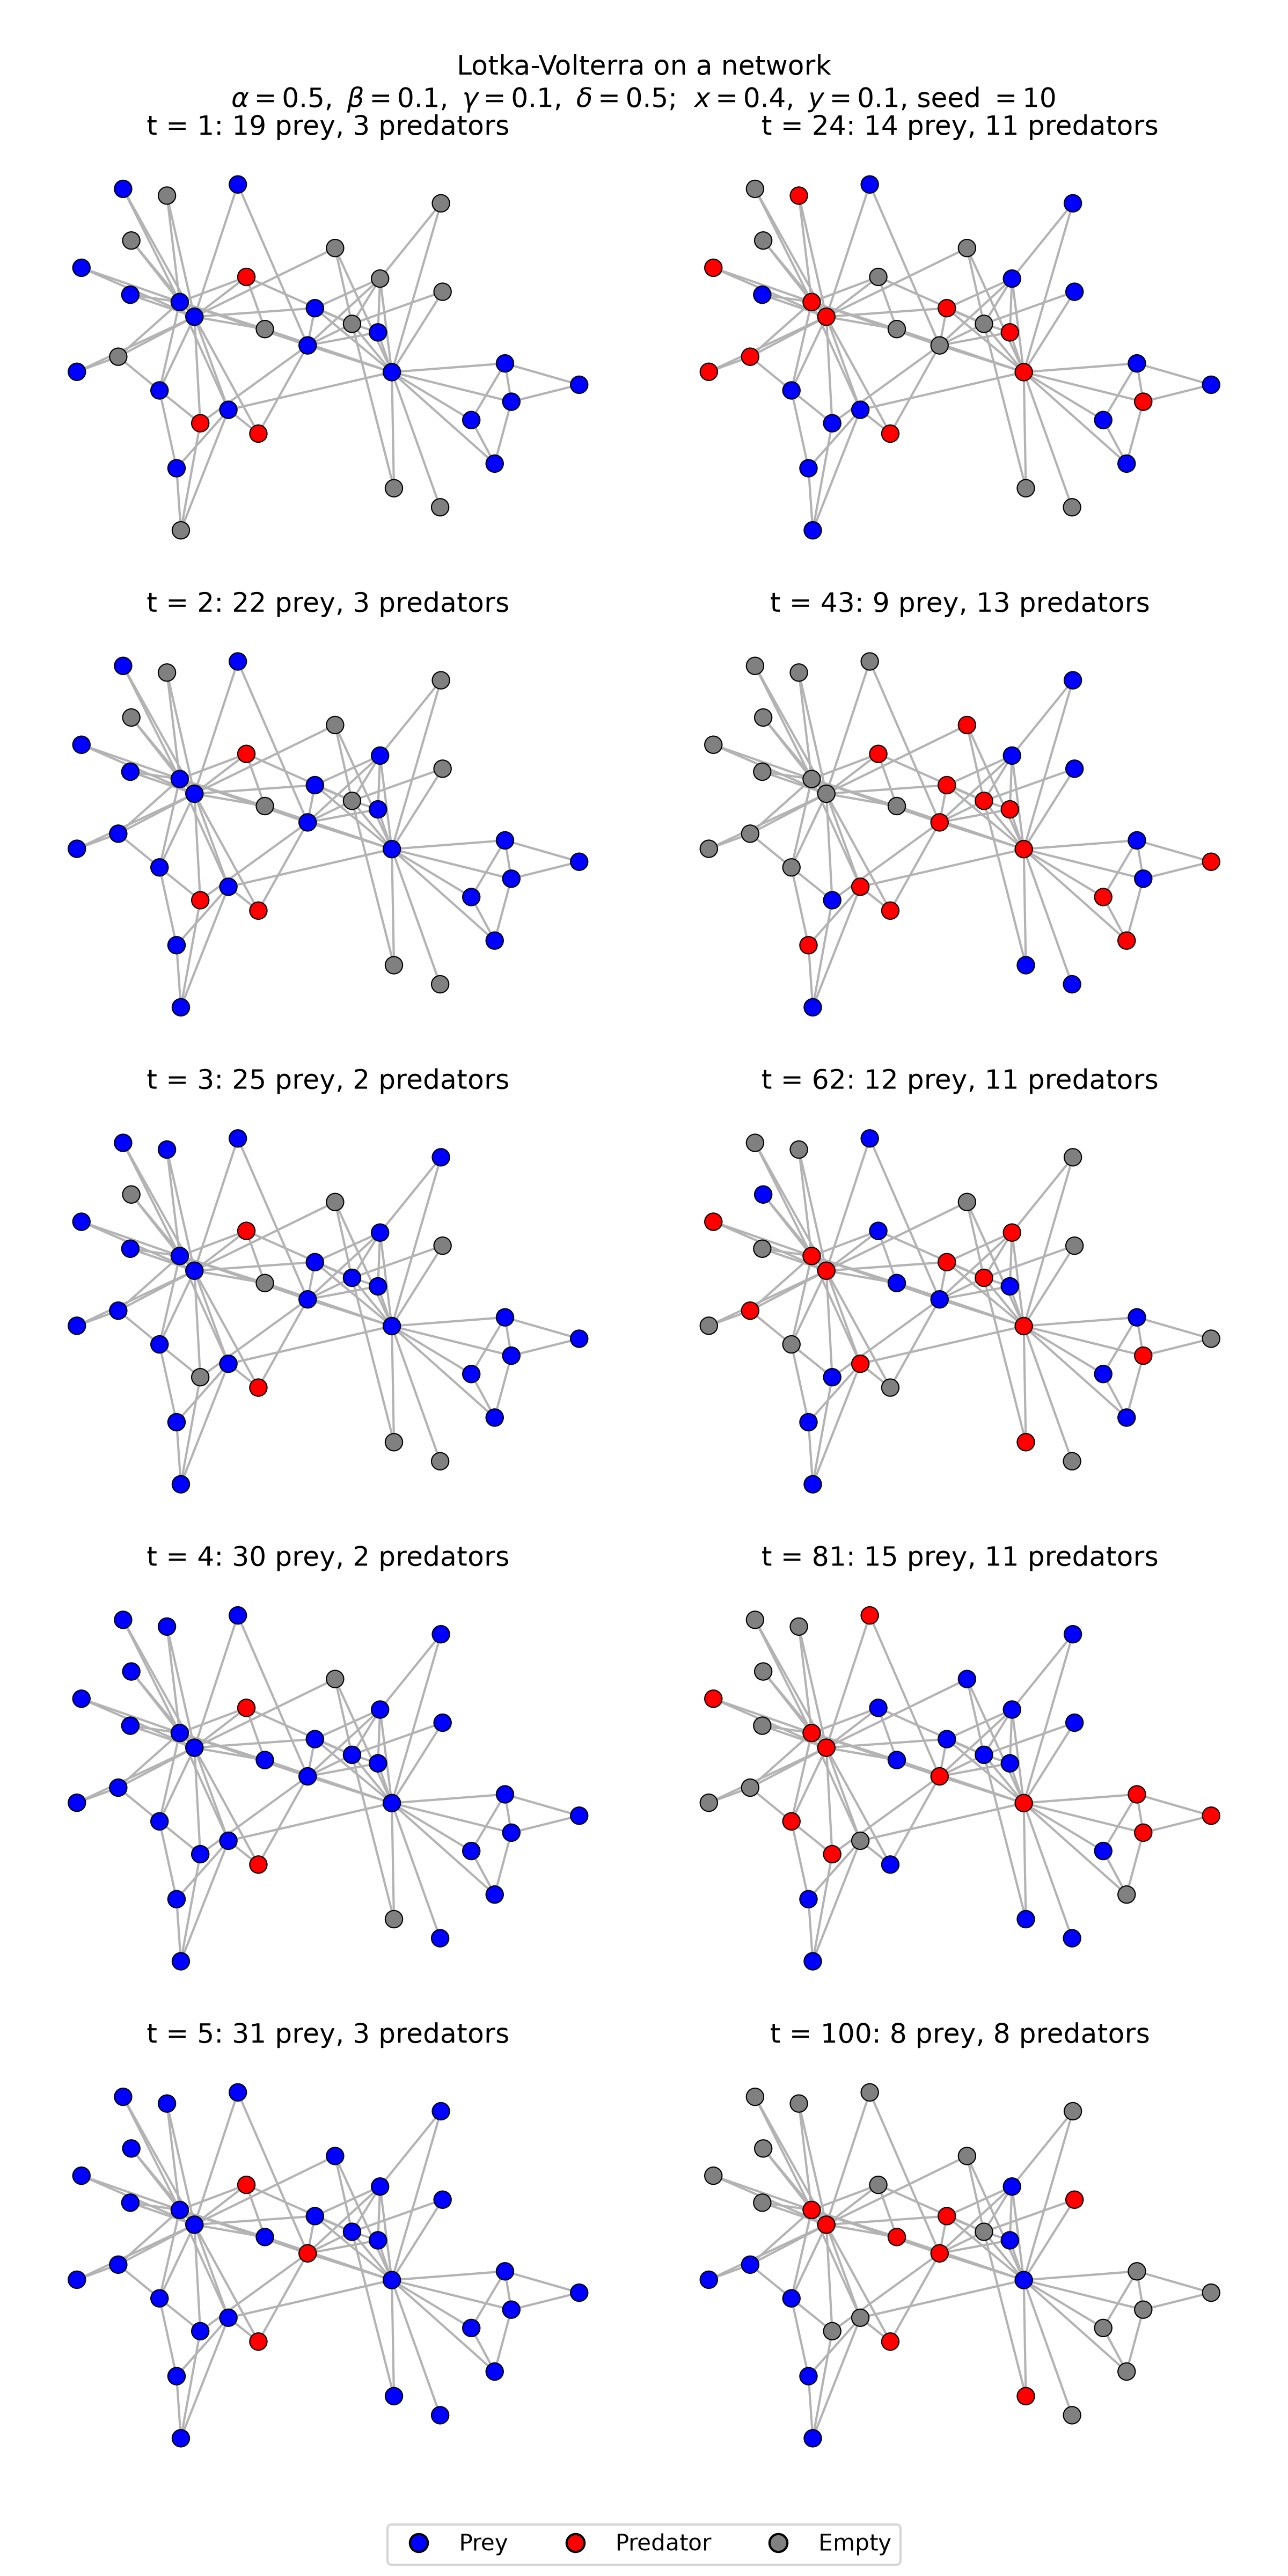
\includegraphics[height=0.8\textheight]{figures/q2a_karate_snapshots.png}
            \caption{Snapshots of the network Lotka-Volterra model on the karate club graph}
            \label{q2aSnapshots}
        \end{figure}
        \begin{figure}[ht!]
            \centering
            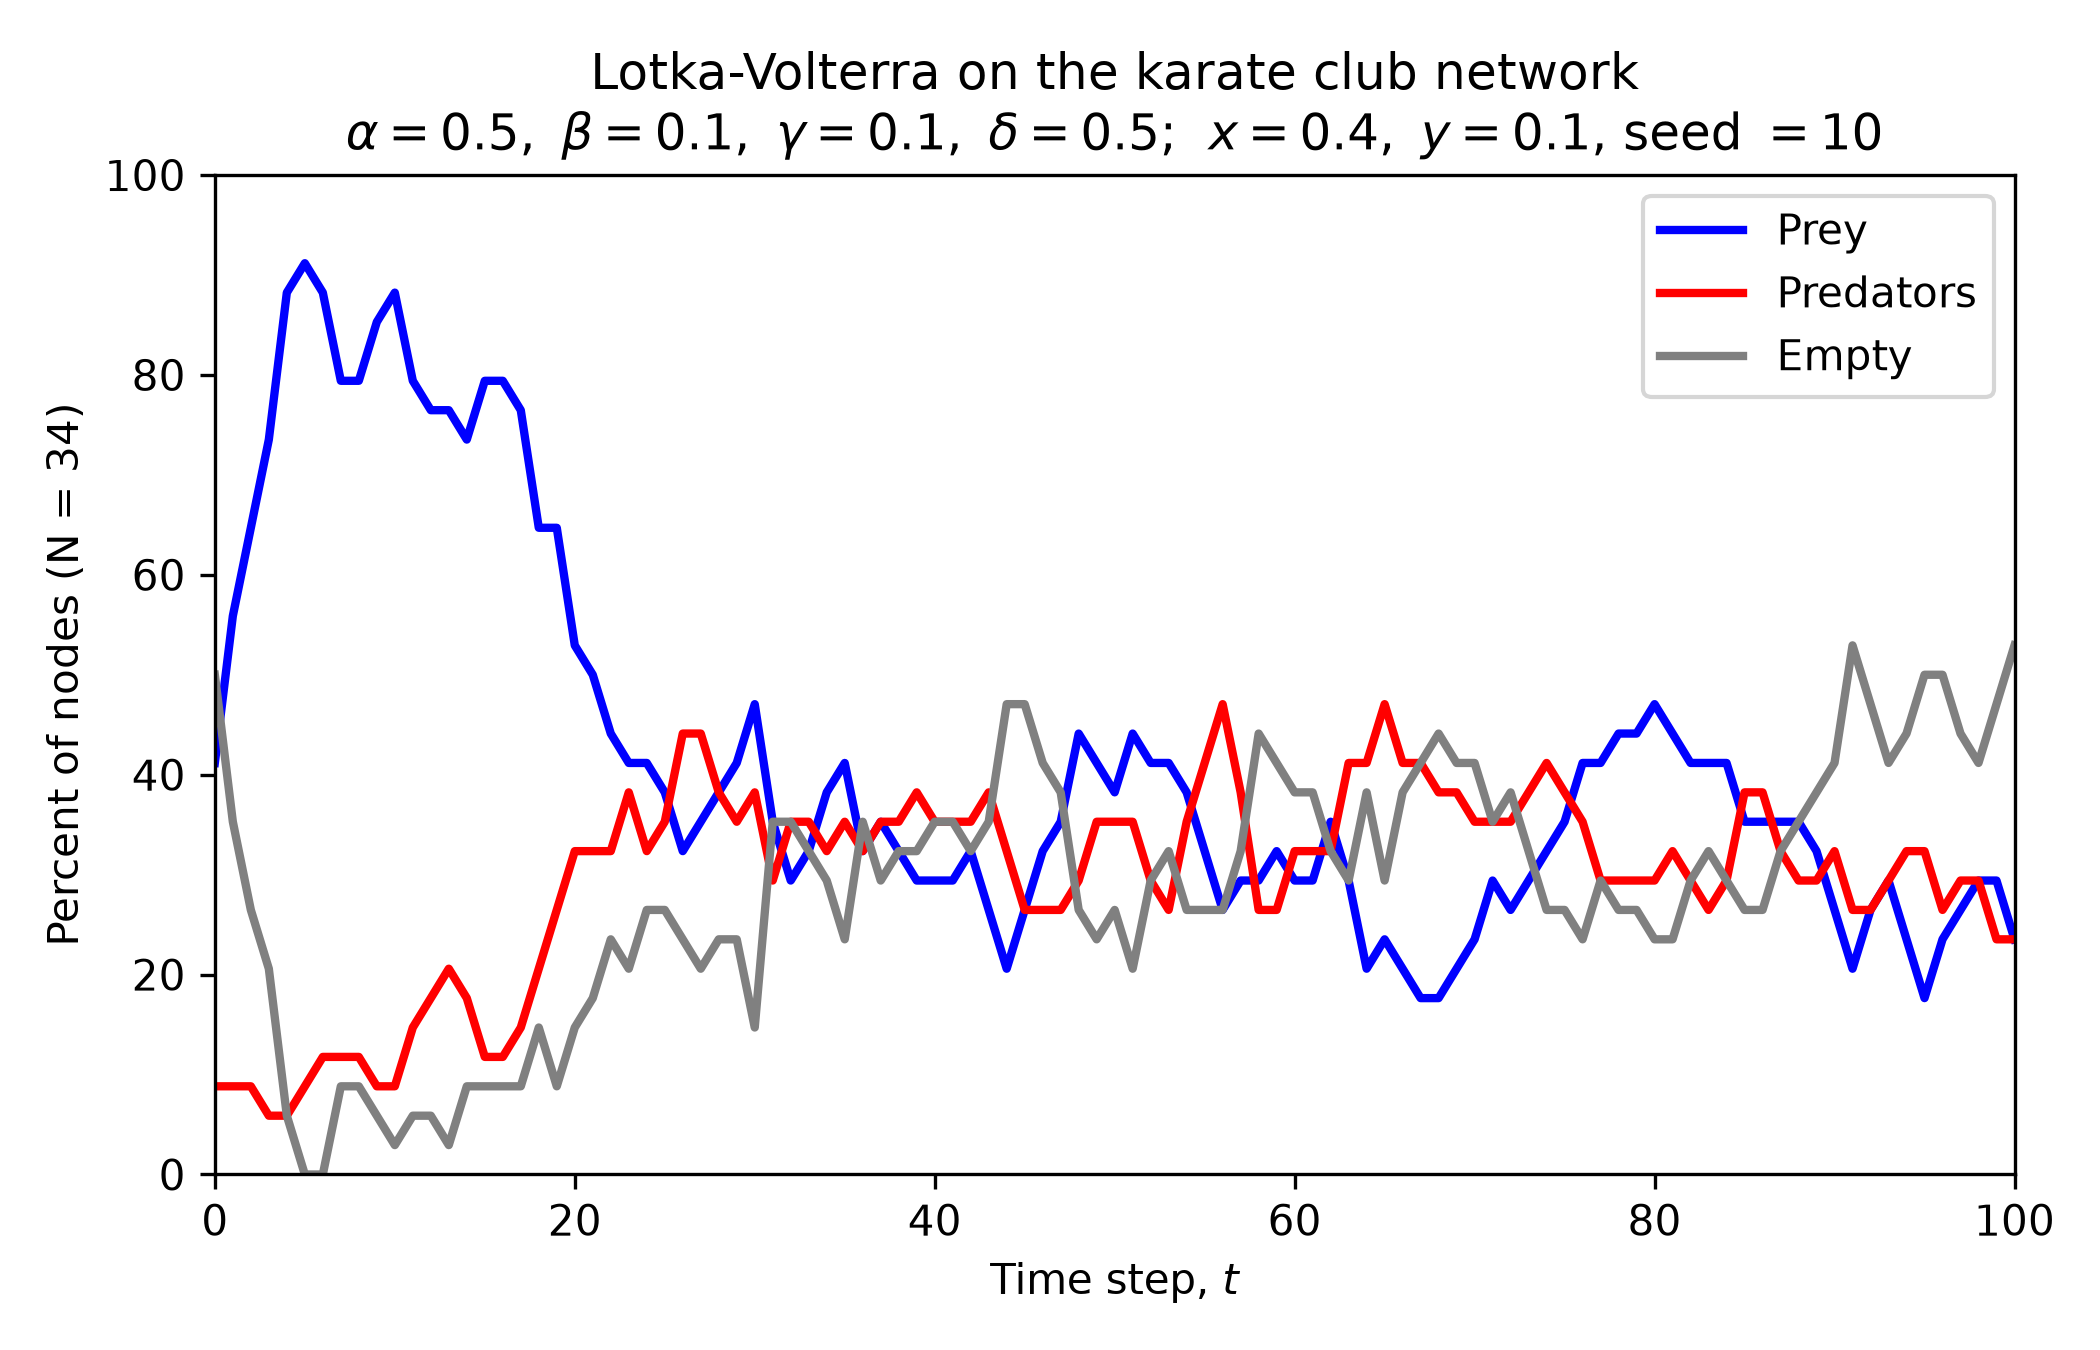
\includegraphics[width=0.85\linewidth]{figures/q2a_karate_populations.png}
            \caption{Prey, predator, and empty populations over time on the karate club graph}
            \label{q2aPopulations}
        \end{figure}

        \item See \texttt{.ipynb}. I built the four graphs as given, adding a seed to the random ones so they are
        reproducible. To compare them fairly, every graph starts with about a third prey, a third predators, and a
        third empty ($x = y = 0.33$), and they all use the karate club rates ($\alpha = 0.5$, $\beta = 0.1$,
        $\gamma = 0.1$, $\delta = 0.5$) for $T = 100$ steps.
        \autoref{q2bPopulations} shows the populations over time for one run (seed 10) of each graph, and
        \autoref{q2bGridSnapshots} and \autoref{q2bArraySnapshots} show the matching snapshots. The lattice is drawn
        on its actual grid positions. For the other three graphs, the 1000 nodes are placed in index order on a fixed
        $20 \times 50$ array with the edges dropped for plotting, so position in those panels is not network
        distance. The exceptions are WS, where index order follows the ring, and BA, where the low-index nodes at the
        top are the oldest nodes and therefore the hubs.
        \begin{itemize}
            \item \textbf{2D grid:} prey quickly take over most of the lattice and the predators hang on in small
            clusters.
            \item \textbf{Erd\H{o}s-R\'enyi:} the predators eat almost all of the prey within the first few steps
            and then starve, leaving every node empty.
            \item \textbf{Barab\'asi-Albert:} the two species coexist, with more prey than predators.
            \item \textbf{Watts-Strogatz:} the predators slowly die out and the prey fill every node.
        \end{itemize}
        Since one run could be a fluke, I also ran each graph 100 times with different simulation seeds (same graph
        each time). \autoref{q2bStatsTable} and \autoref{q2bHistograms} summarize the final populations at $t = 100$.
        The seed 10 runs above turn out to be typical. The grid is extremely consistent (SD under 1\%), ER almost
        always ends in total extinction (though in a few runs some predators are still alive at $t=100$), BA
        coexists with the widest spread, and WS ends with the prey taking over in every run.
        \begin{figure}[ht!]
            \centering
            \begin{minipage}{0.49\linewidth}
                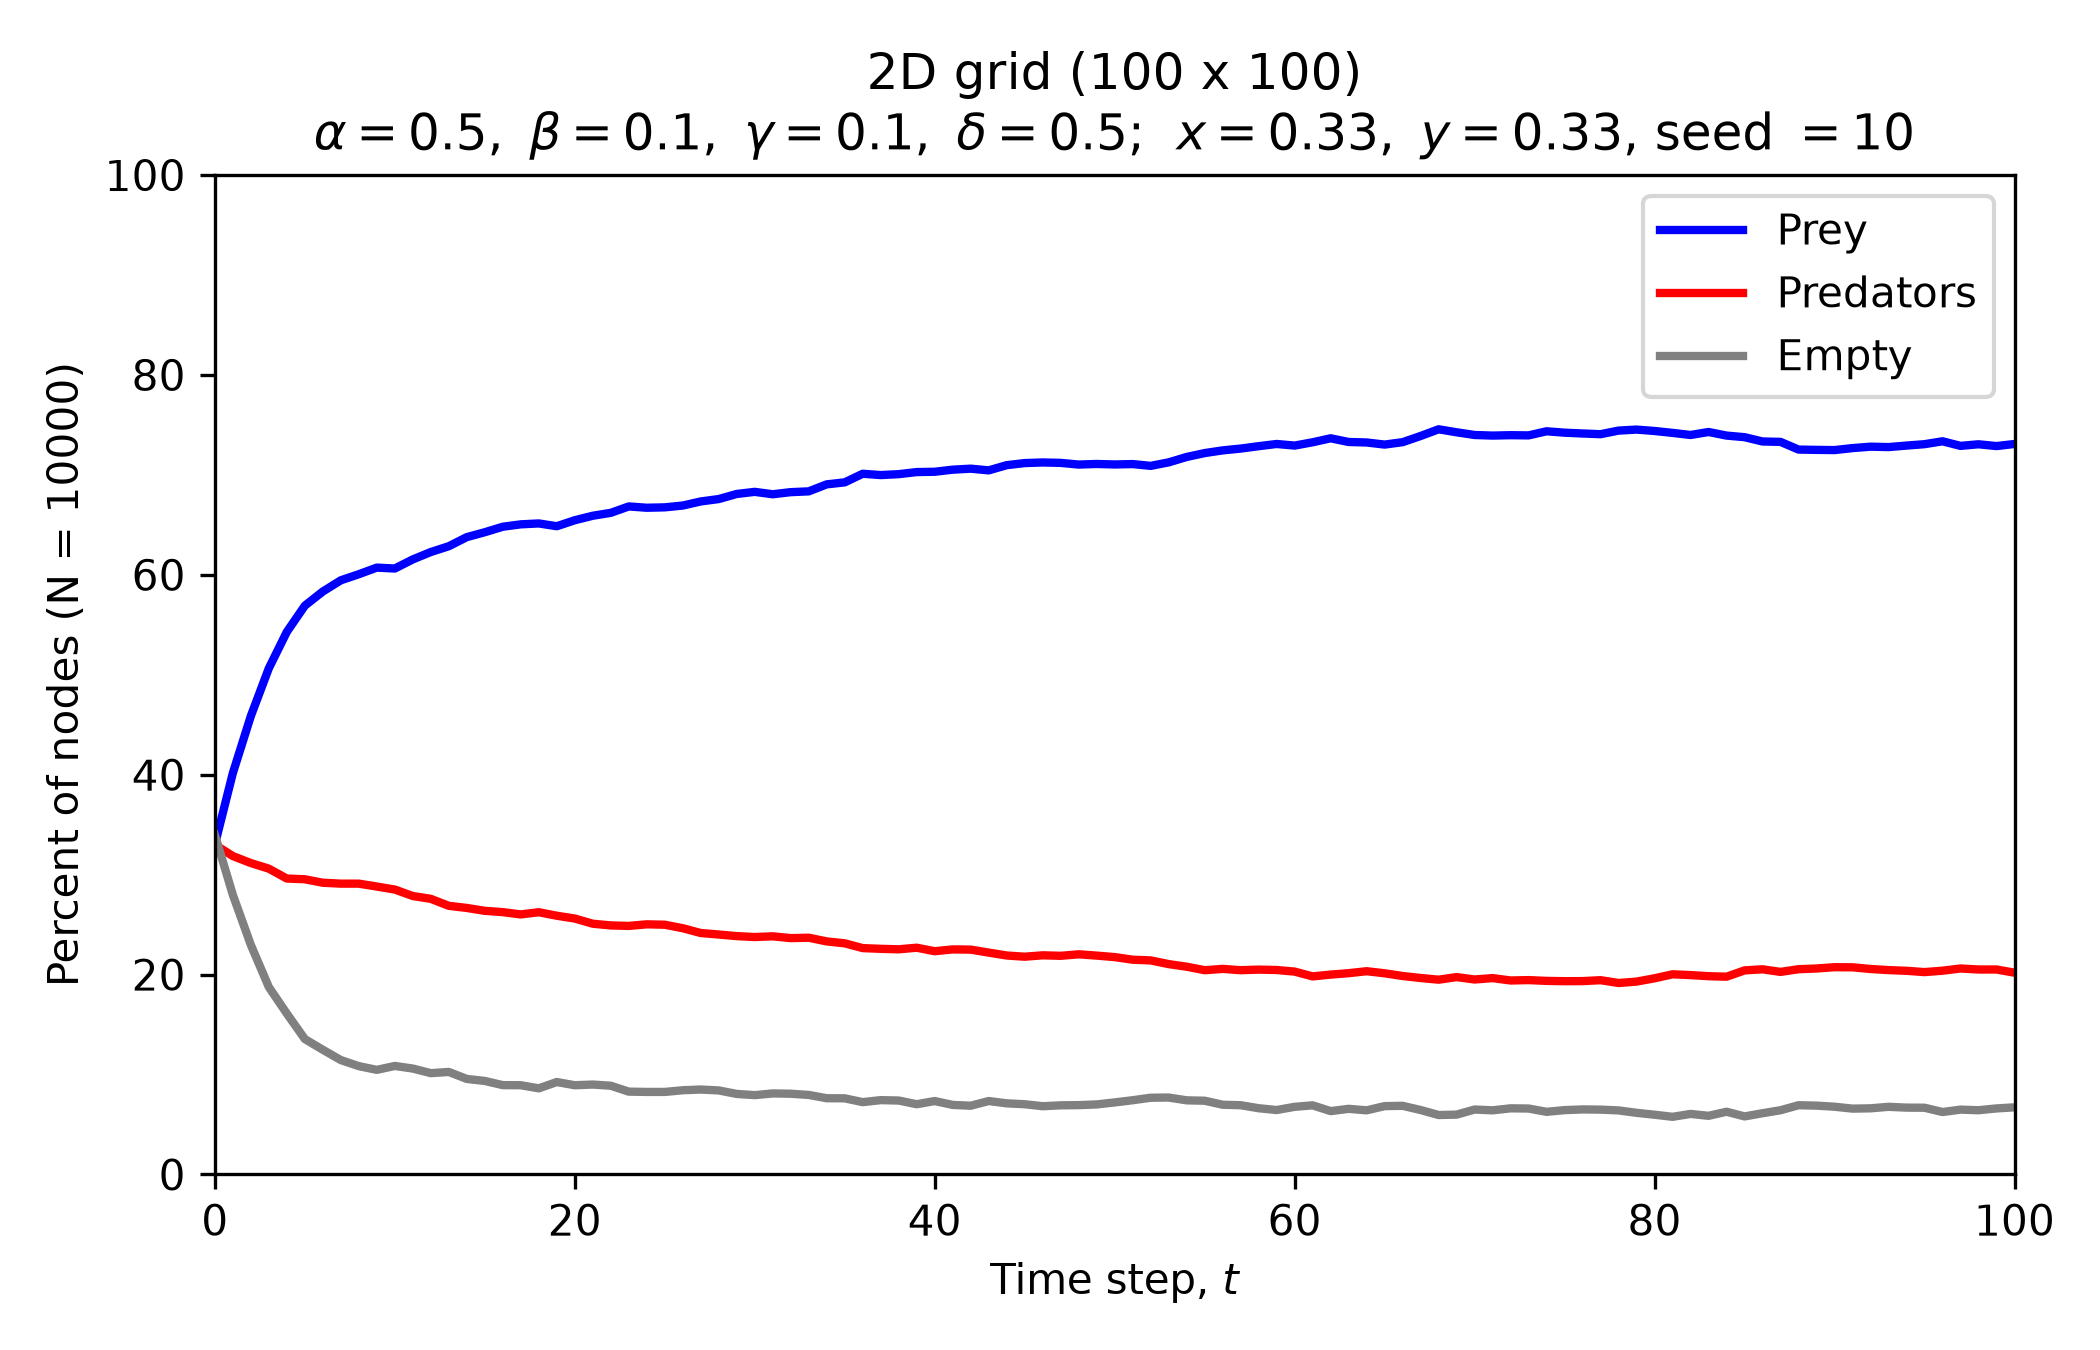
\includegraphics[width=\linewidth]{figures/q2b_grid.png}
            \end{minipage}\hfill
            \begin{minipage}{0.49\linewidth}
                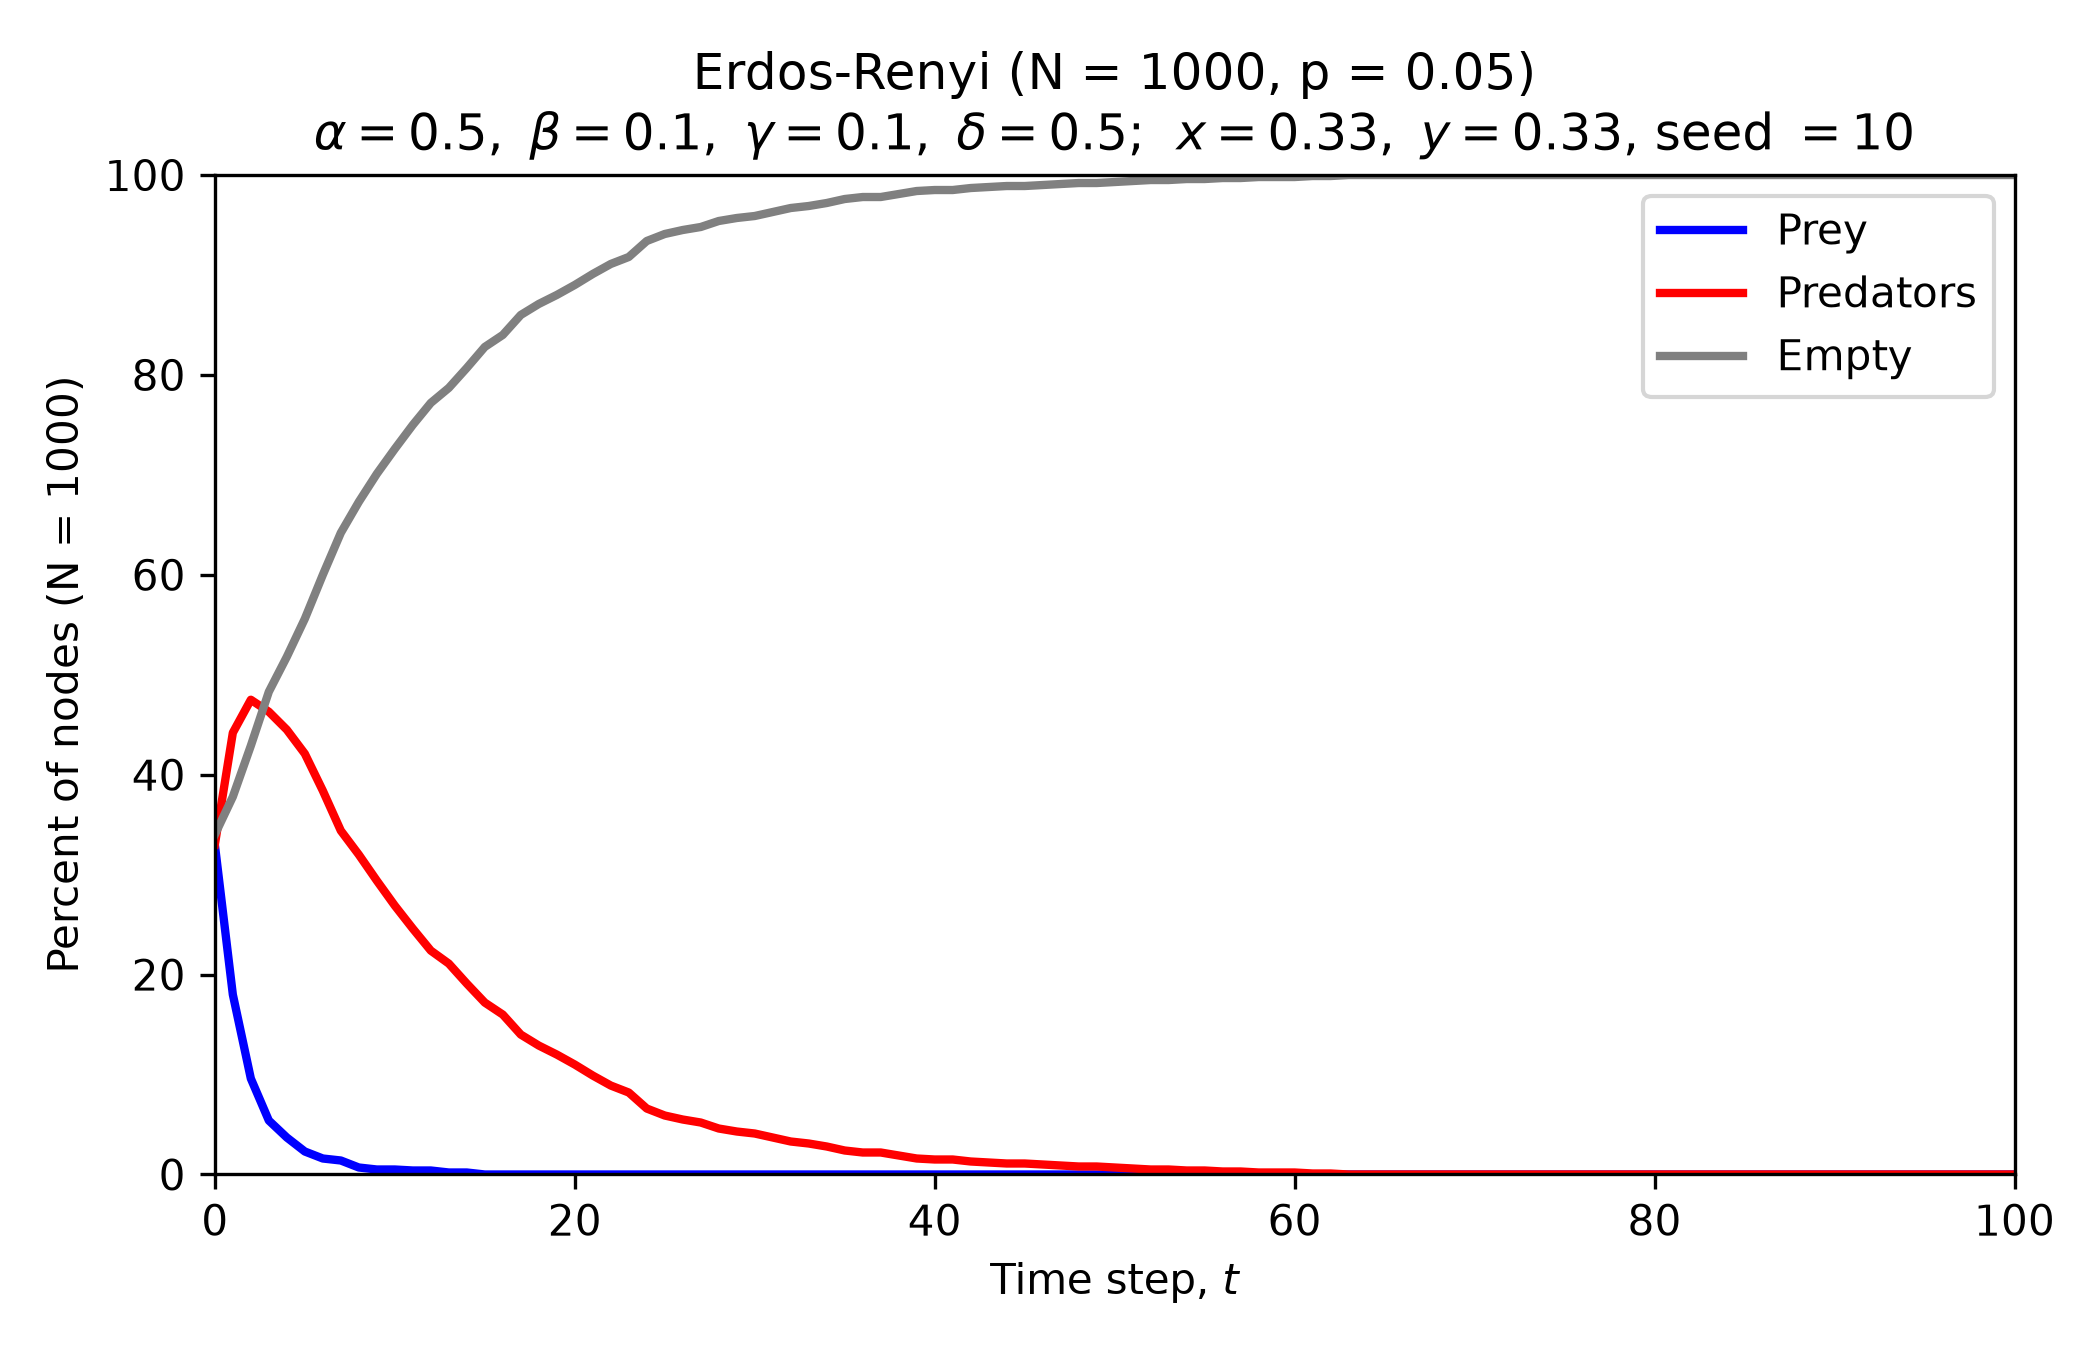
\includegraphics[width=\linewidth]{figures/q2b_erdos_renyi.png}
            \end{minipage}\\[6pt]
            \begin{minipage}{0.49\linewidth}
                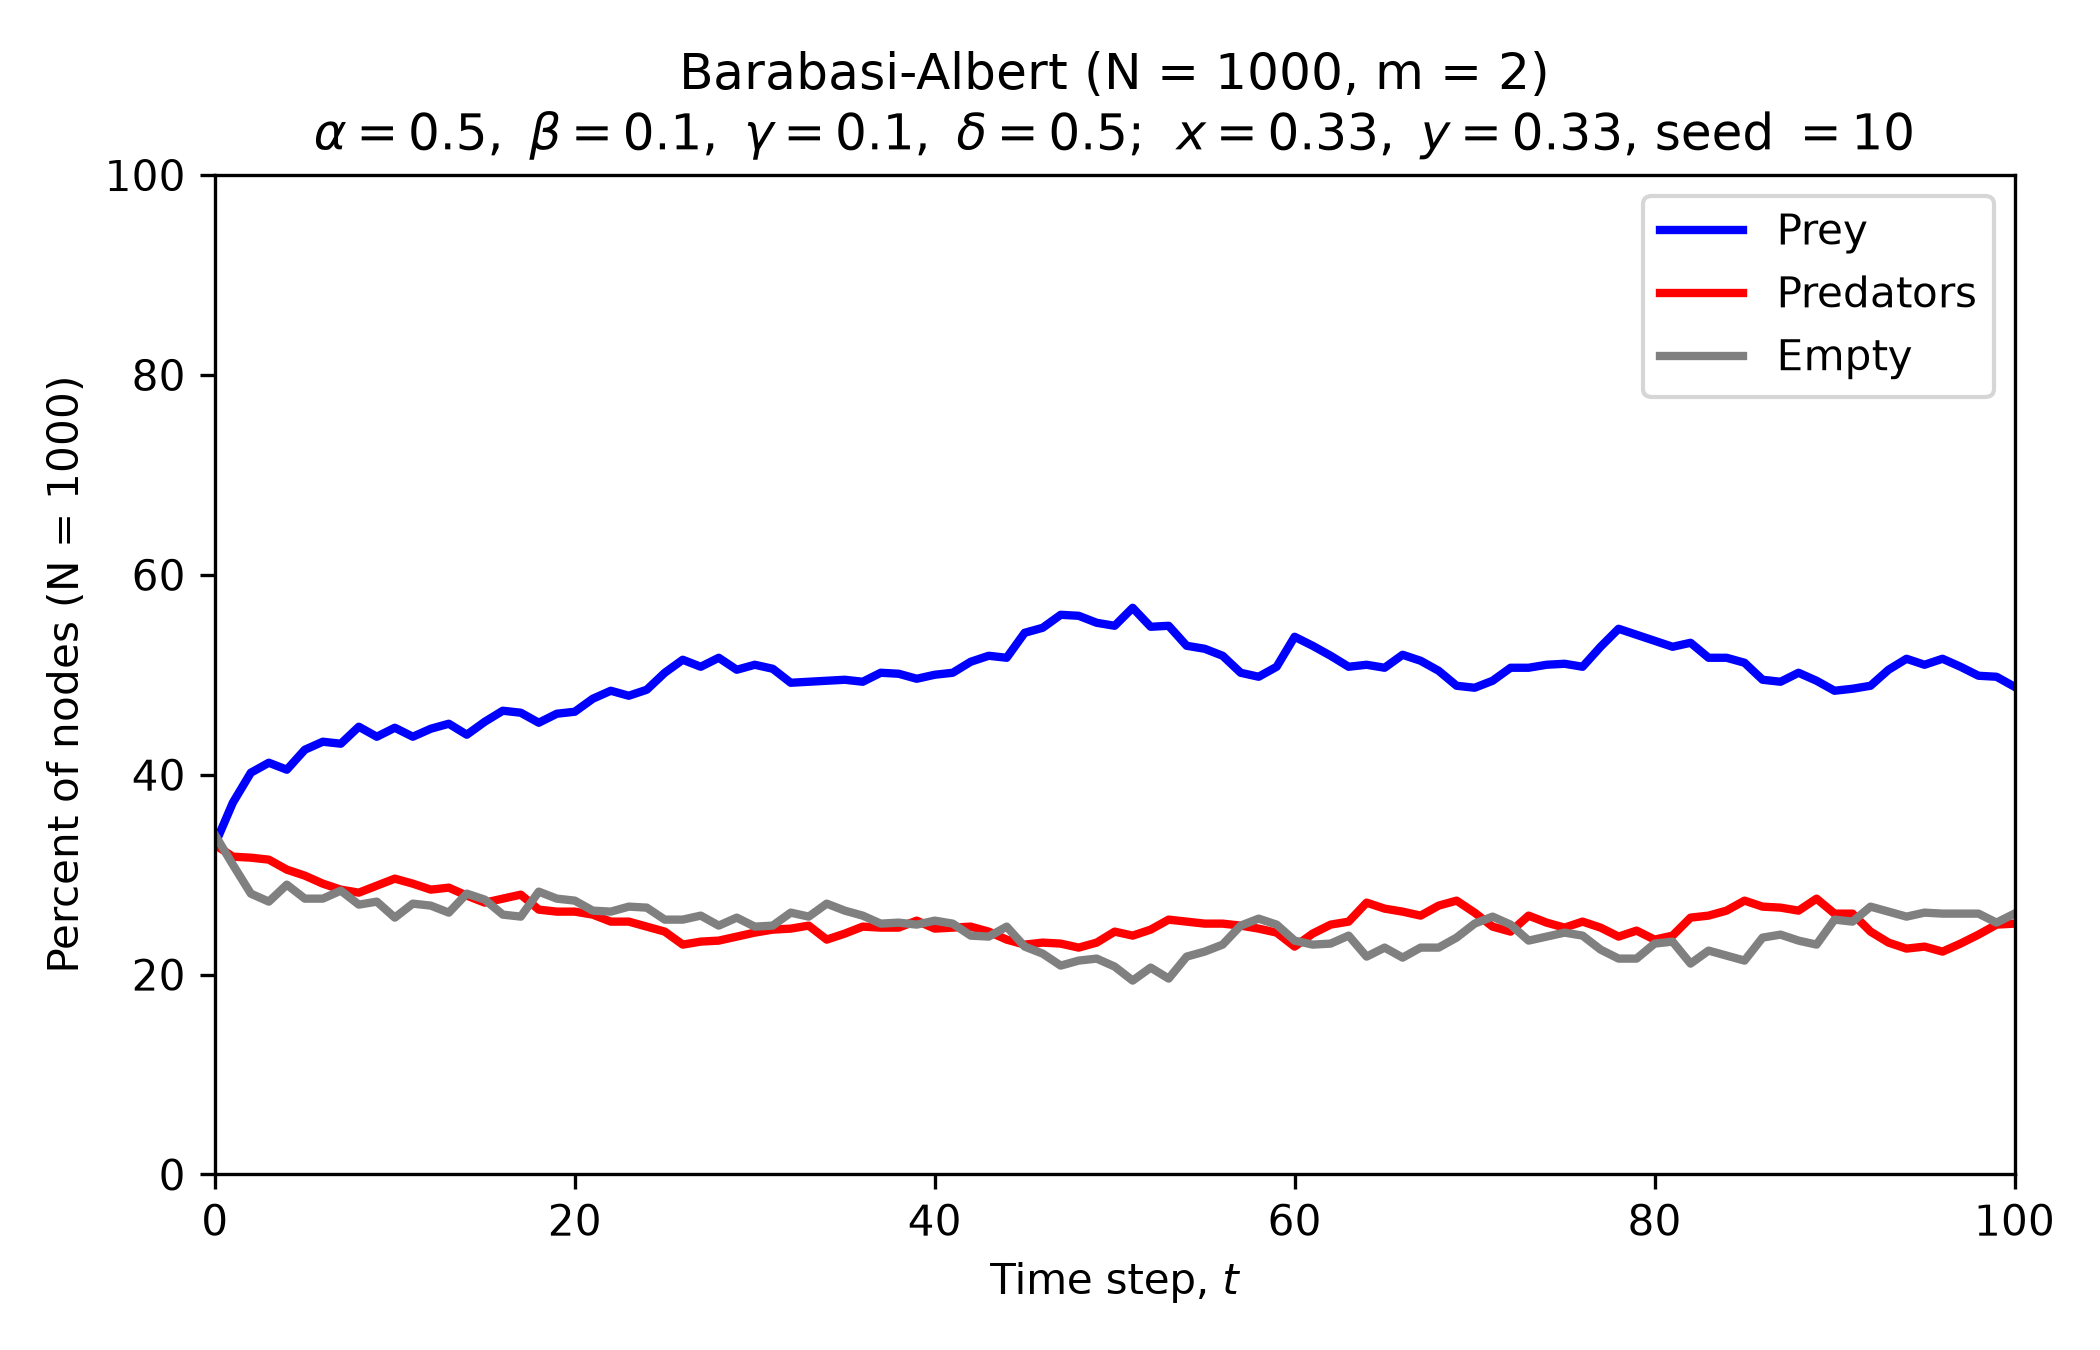
\includegraphics[width=\linewidth]{figures/q2b_barabasi_albert.png}
            \end{minipage}\hfill
            \begin{minipage}{0.49\linewidth}
                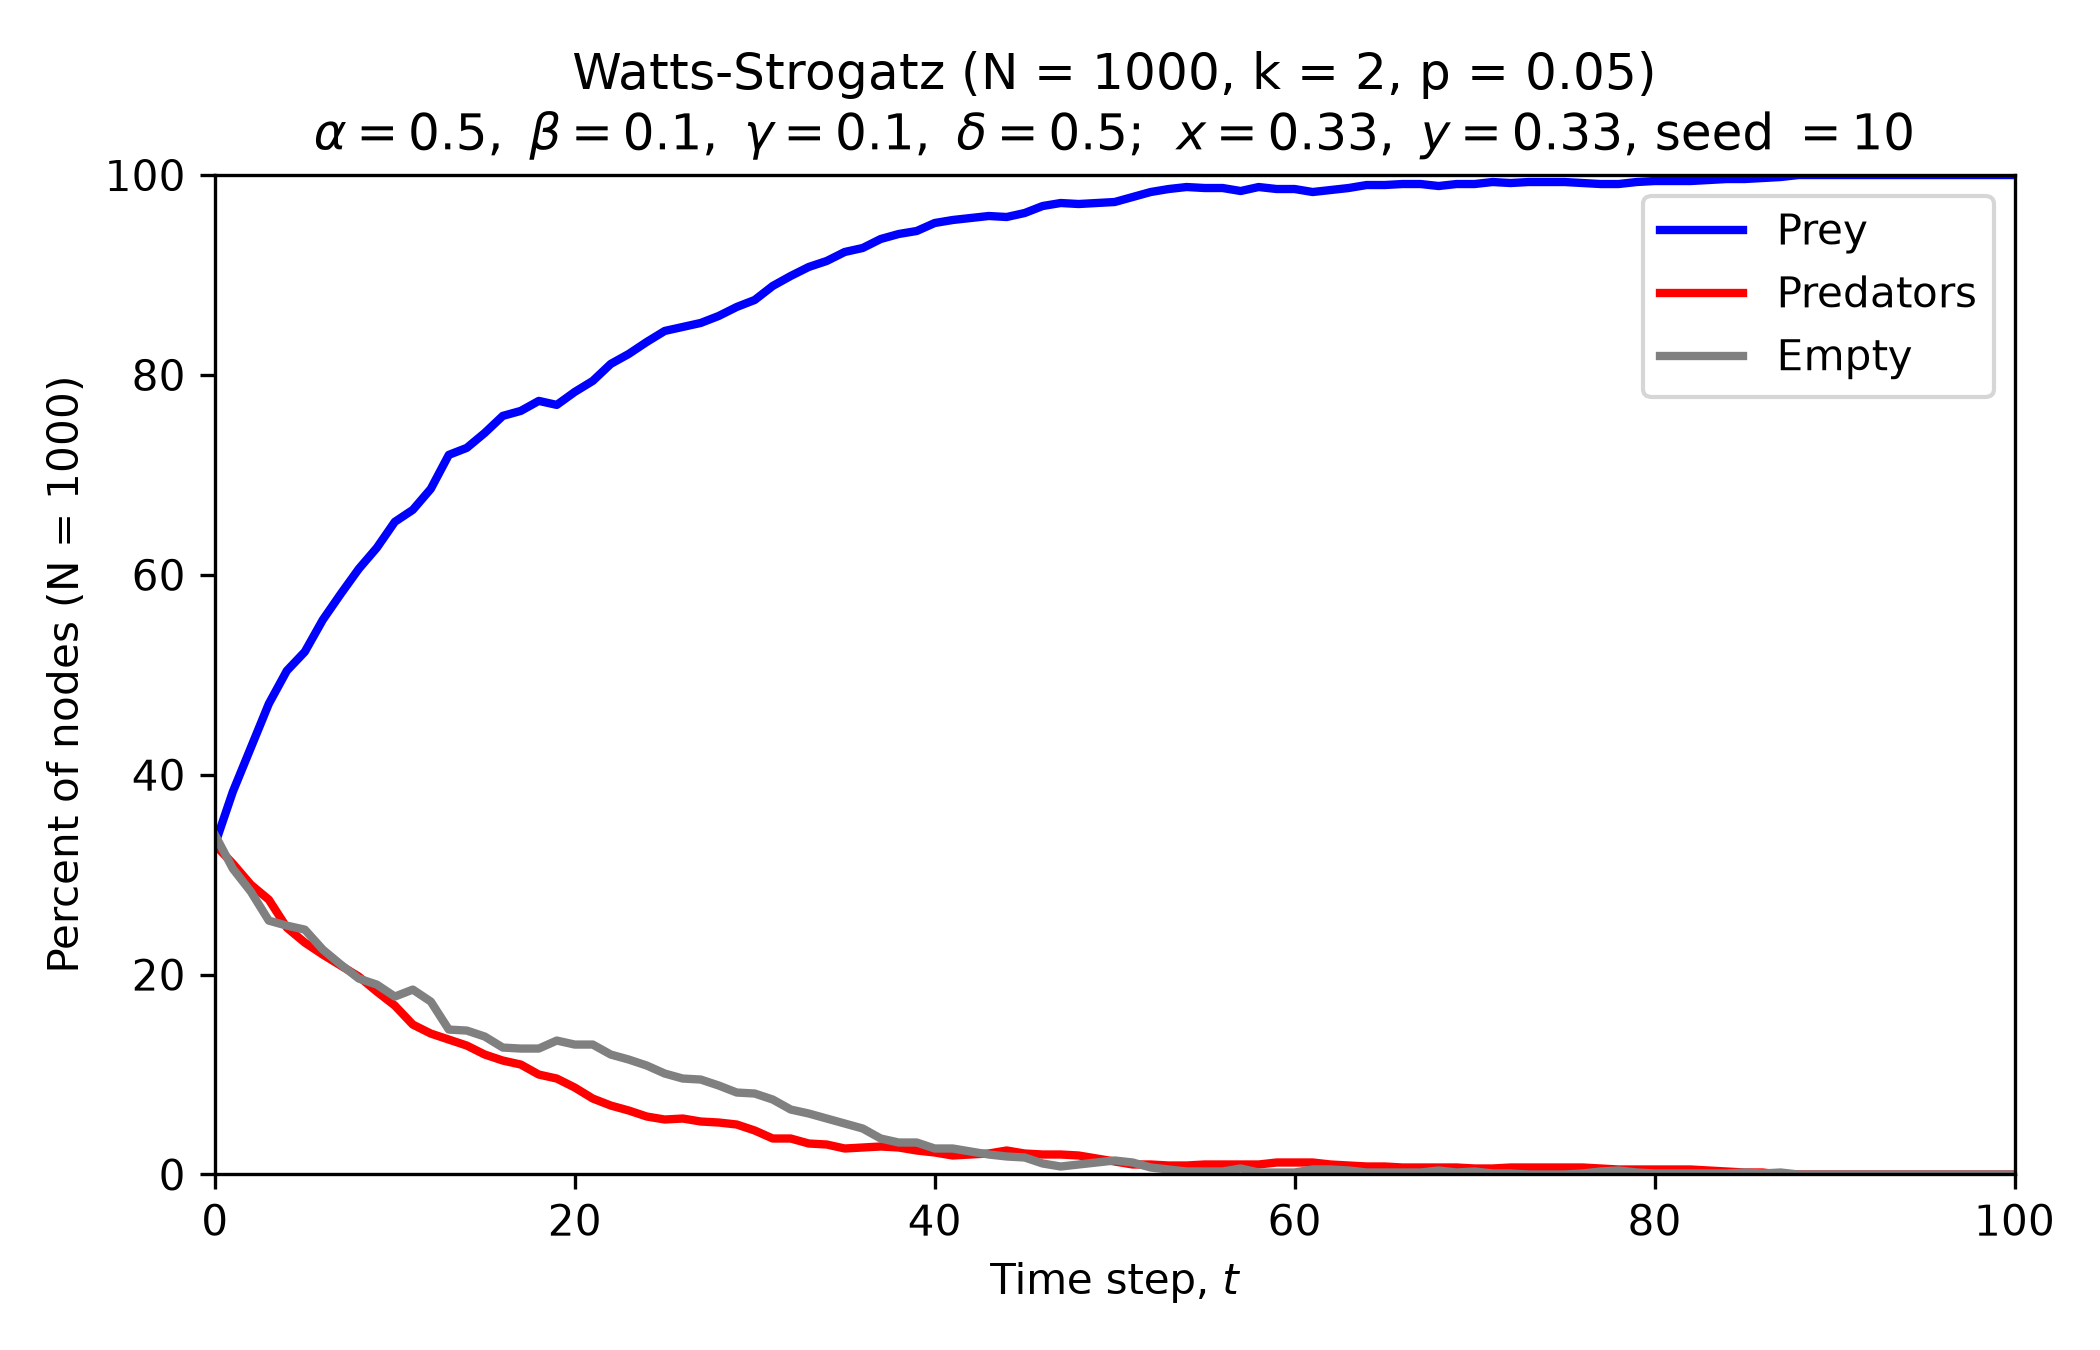
\includegraphics[width=\linewidth]{figures/q2b_watts_strogatz.png}
            \end{minipage}
            \caption{Populations over time on the four graphs (seed 10), $x = y = 0.33$}
            \label{q2bPopulations}
        \end{figure}
        \begin{figure}[ht!]
            \centering
            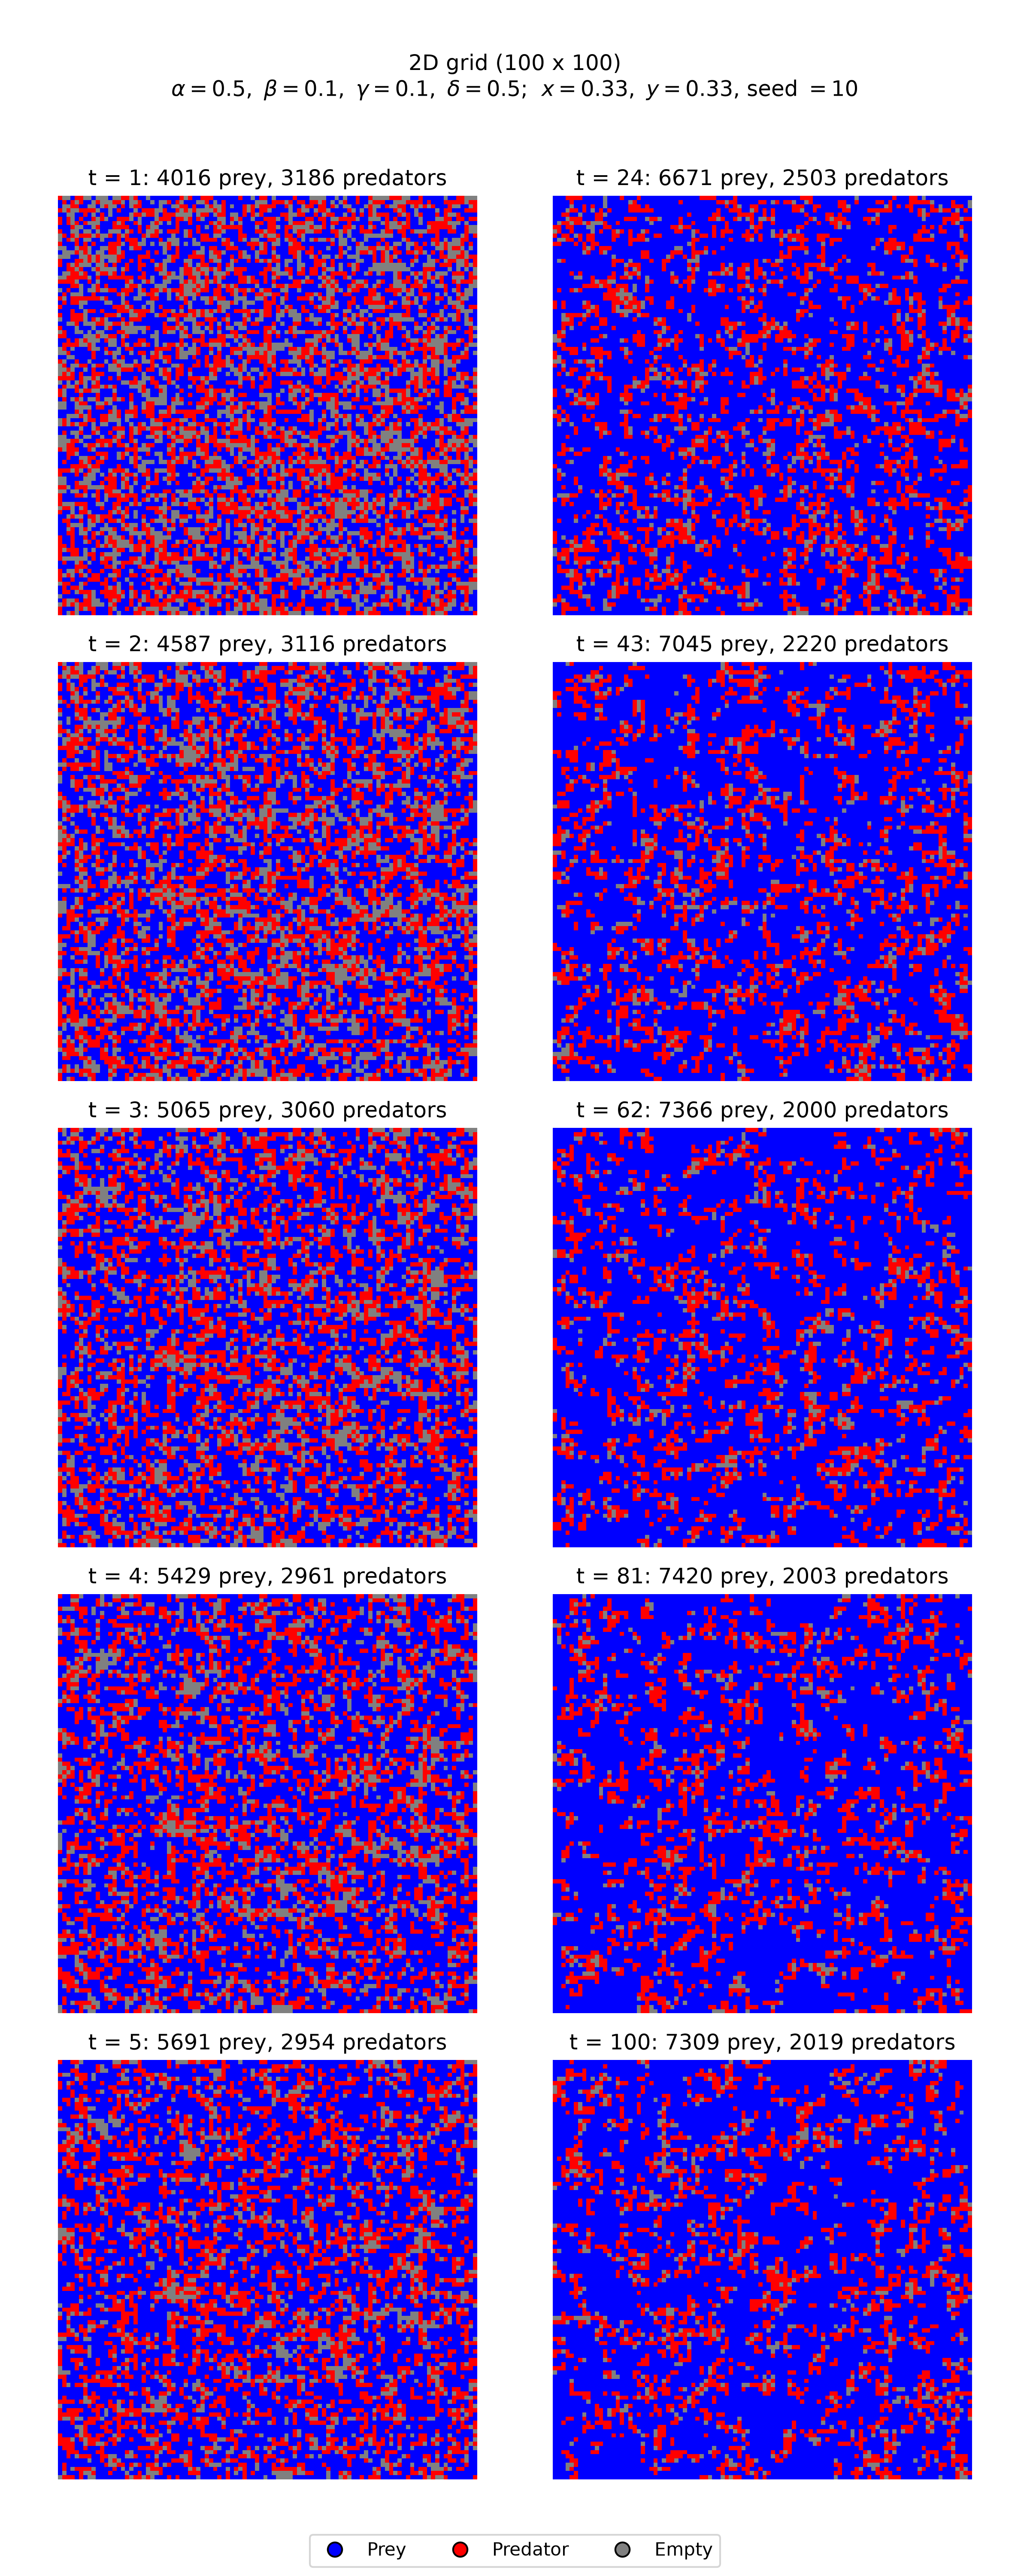
\includegraphics[height=0.85\textheight]{figures/q2b_grid_snapshots.png}
            \caption{Snapshots on the $100 \times 100$ grid (seed 10)}
            \label{q2bGridSnapshots}
        \end{figure}
        \begin{figure}[ht!]
            \centering
            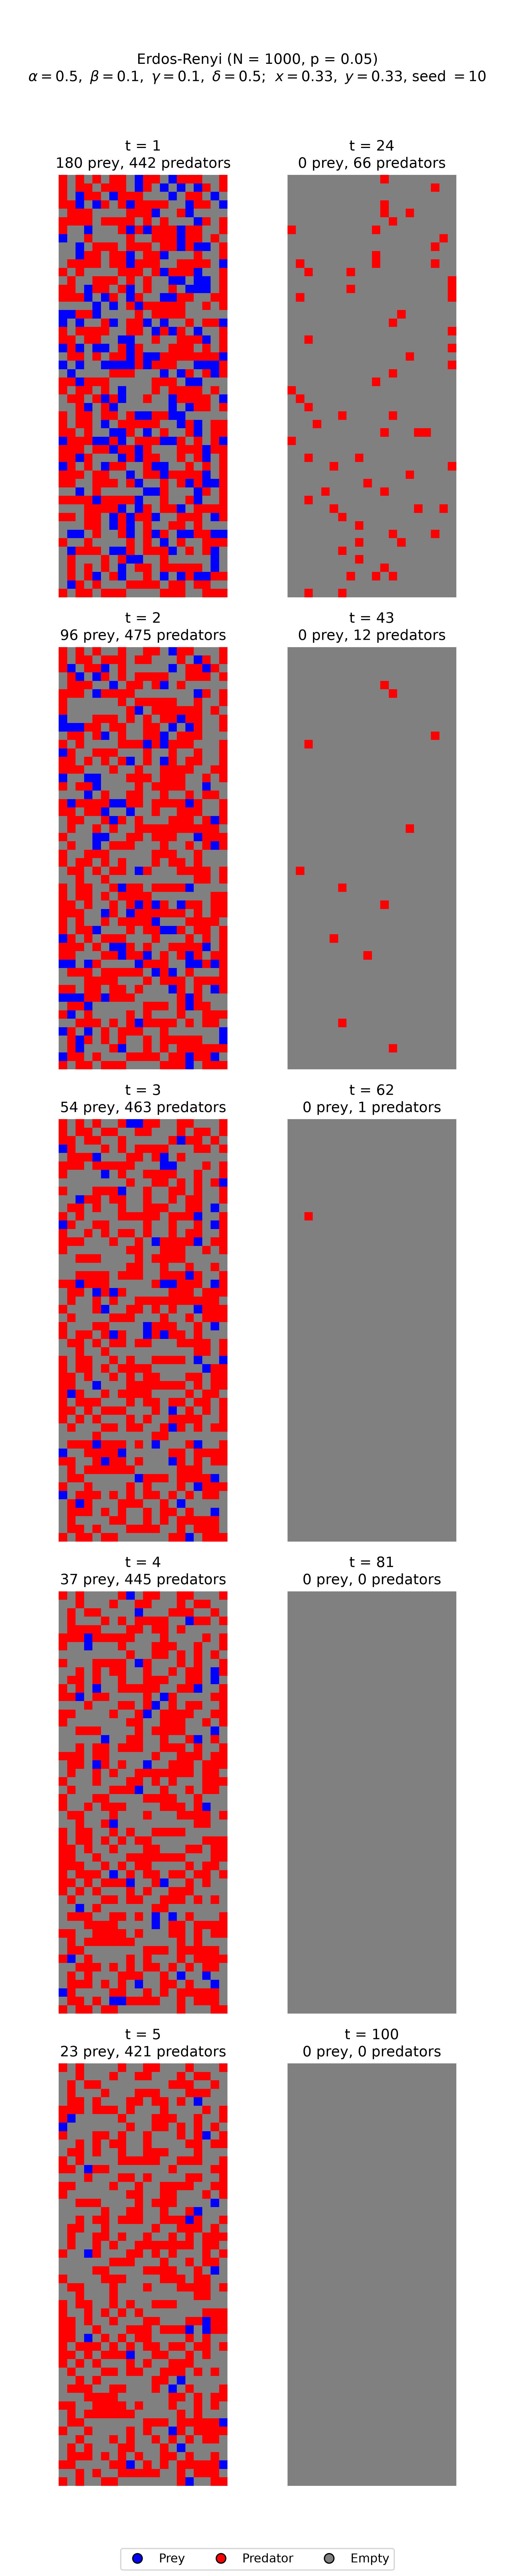
\includegraphics[height=0.8\textheight]{figures/q2b_erdos_renyi_snapshots.png}\hfill
            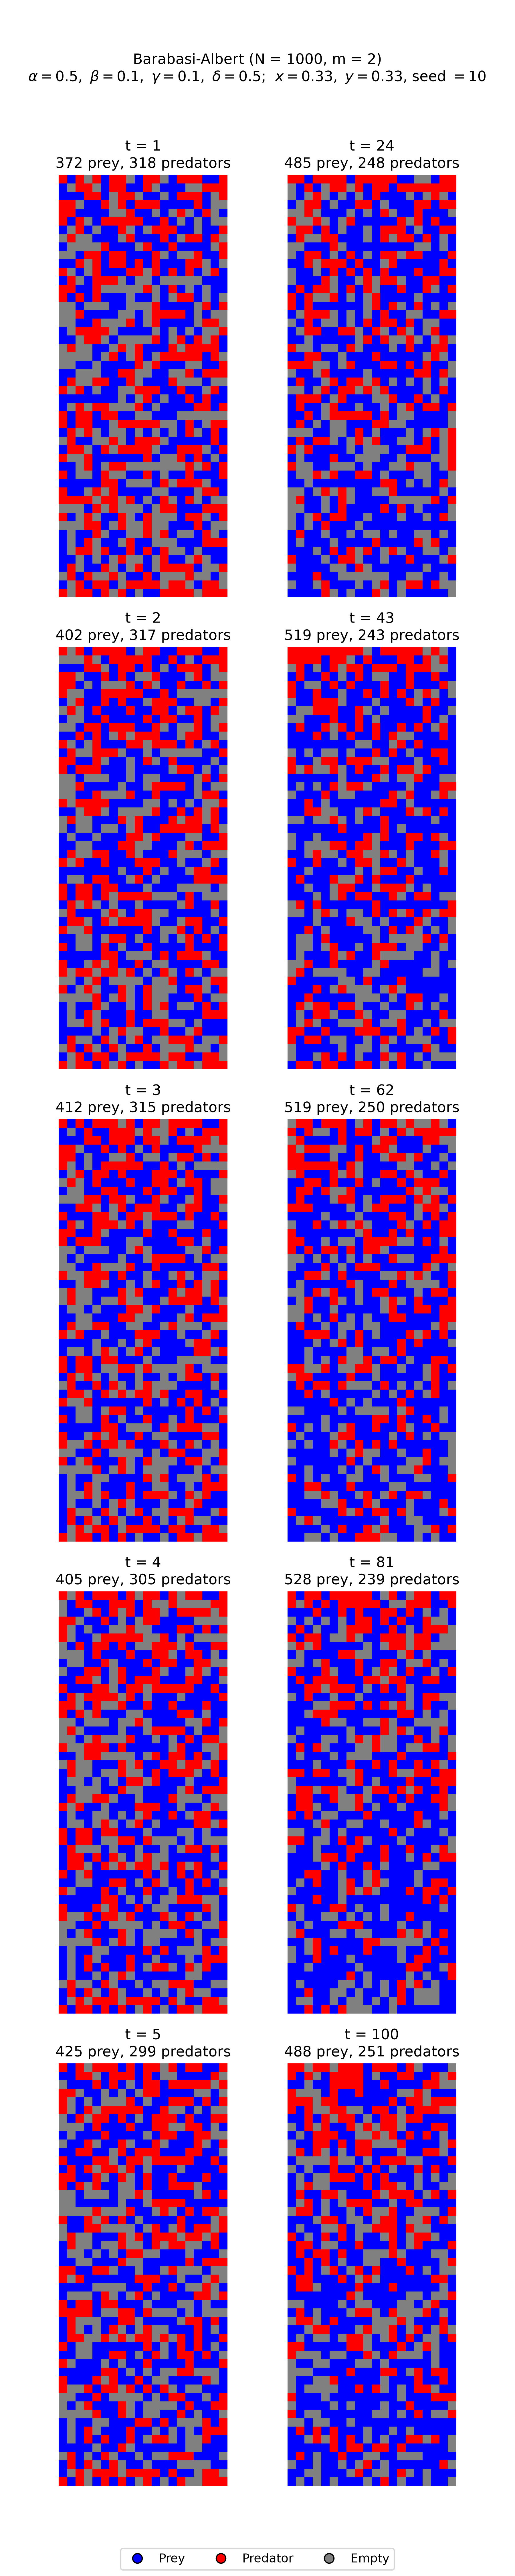
\includegraphics[height=0.8\textheight]{figures/q2b_barabasi_albert_snapshots.png}\hfill
            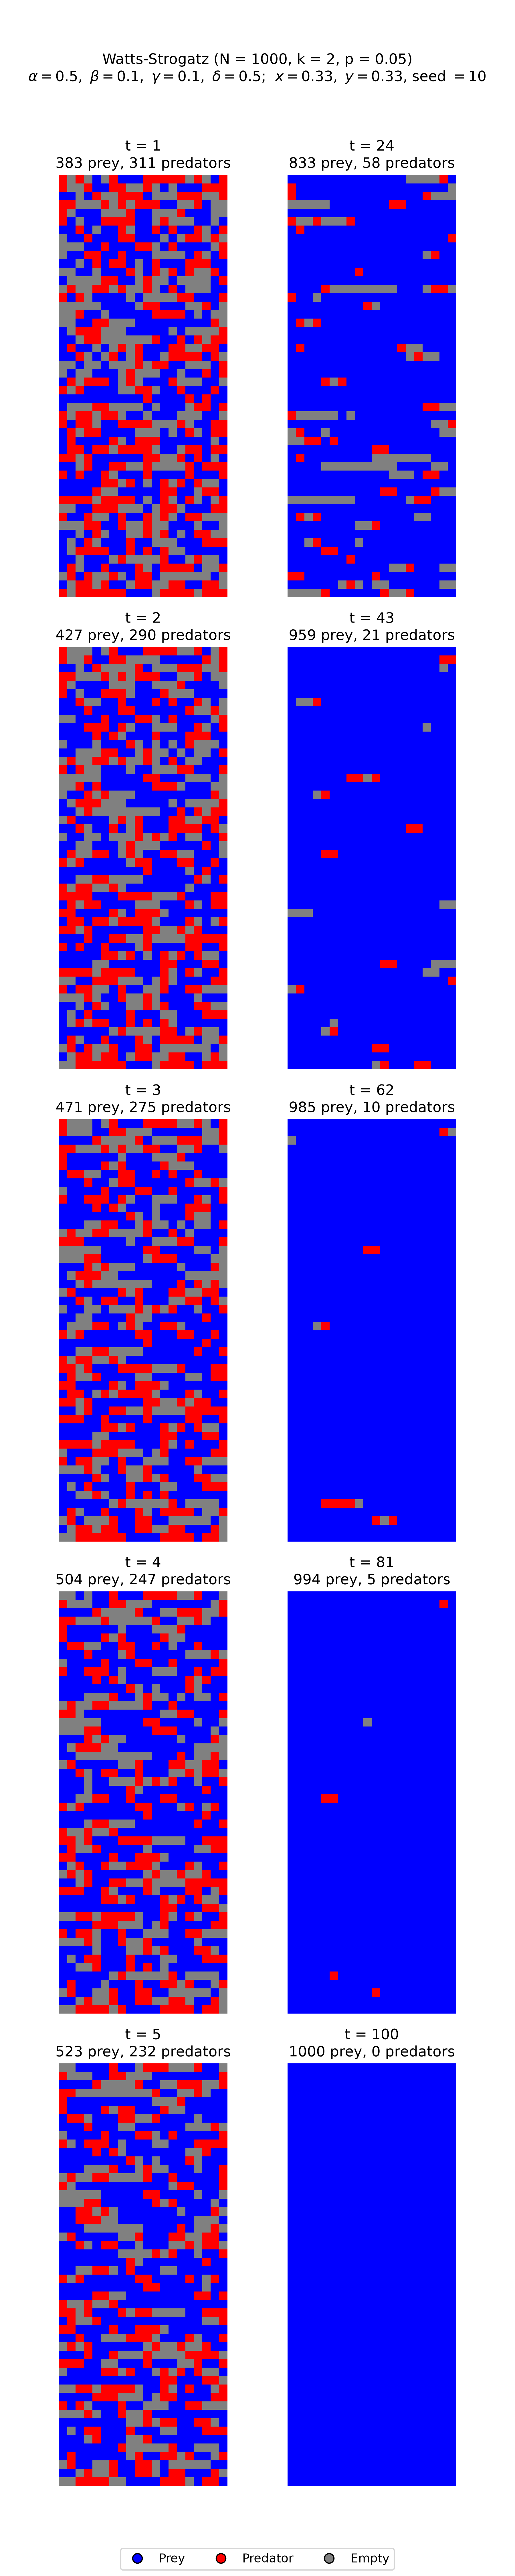
\includegraphics[height=0.8\textheight]{figures/q2b_watts_strogatz_snapshots.png}
            \caption{Snapshots on (left to right) ER, BA, and WS (seed 10), nodes in index order on a $20 \times 50$ array, edges dropped for plotting}
            \label{q2bArraySnapshots}
        \end{figure}
        \begin{table}[ht!]
            \centering
            \begin{tabular}{llrrrr}
                \toprule
                Graph & Population & Mean & Median & Mode & SD \\
                \midrule
                2D grid & Prey & 75.67 & 75.76 & 74.87 & 0.99 \\
                 & Predators & 18.38 & 18.32 & 17.63 & 0.75 \\
                 & Empty & 5.95 & 5.95 & 5.68 & 0.35 \\
                \midrule
                Erd\H{o}s-R\'enyi & Prey & 0.47 & 0.00 & 0.00 & 1.13 \\
                 & Predators & 2.41 & 0.00 & 0.00 & 4.90 \\
                 & Empty & 97.12 & 100.00 & 100.00 & 5.62 \\
                \midrule
                Barab\'asi-Albert & Prey & 51.82 & 51.75 & 54.50 & 3.18 \\
                 & Predators & 24.52 & 24.65 & 24.70 & 1.60 \\
                 & Empty & 23.65 & 23.75 & 23.90 & 2.25 \\
                \midrule
                Watts-Strogatz & Prey & 99.73 & 99.85 & 100.00 & 0.34 \\
                 & Predators & 0.16 & 0.10 & 0.00 & 0.20 \\
                 & Empty & 0.12 & 0.00 & 0.00 & 0.21 \\
                \bottomrule
            \end{tabular}
            \caption{Final populations at $t = 100$ (\% of nodes) over 100 runs per graph. Mode is the most common exact final value and SD is the sample standard deviation.}
            \label{q2bStatsTable}
        \end{table}
        \begin{figure}[ht!]
            \centering
            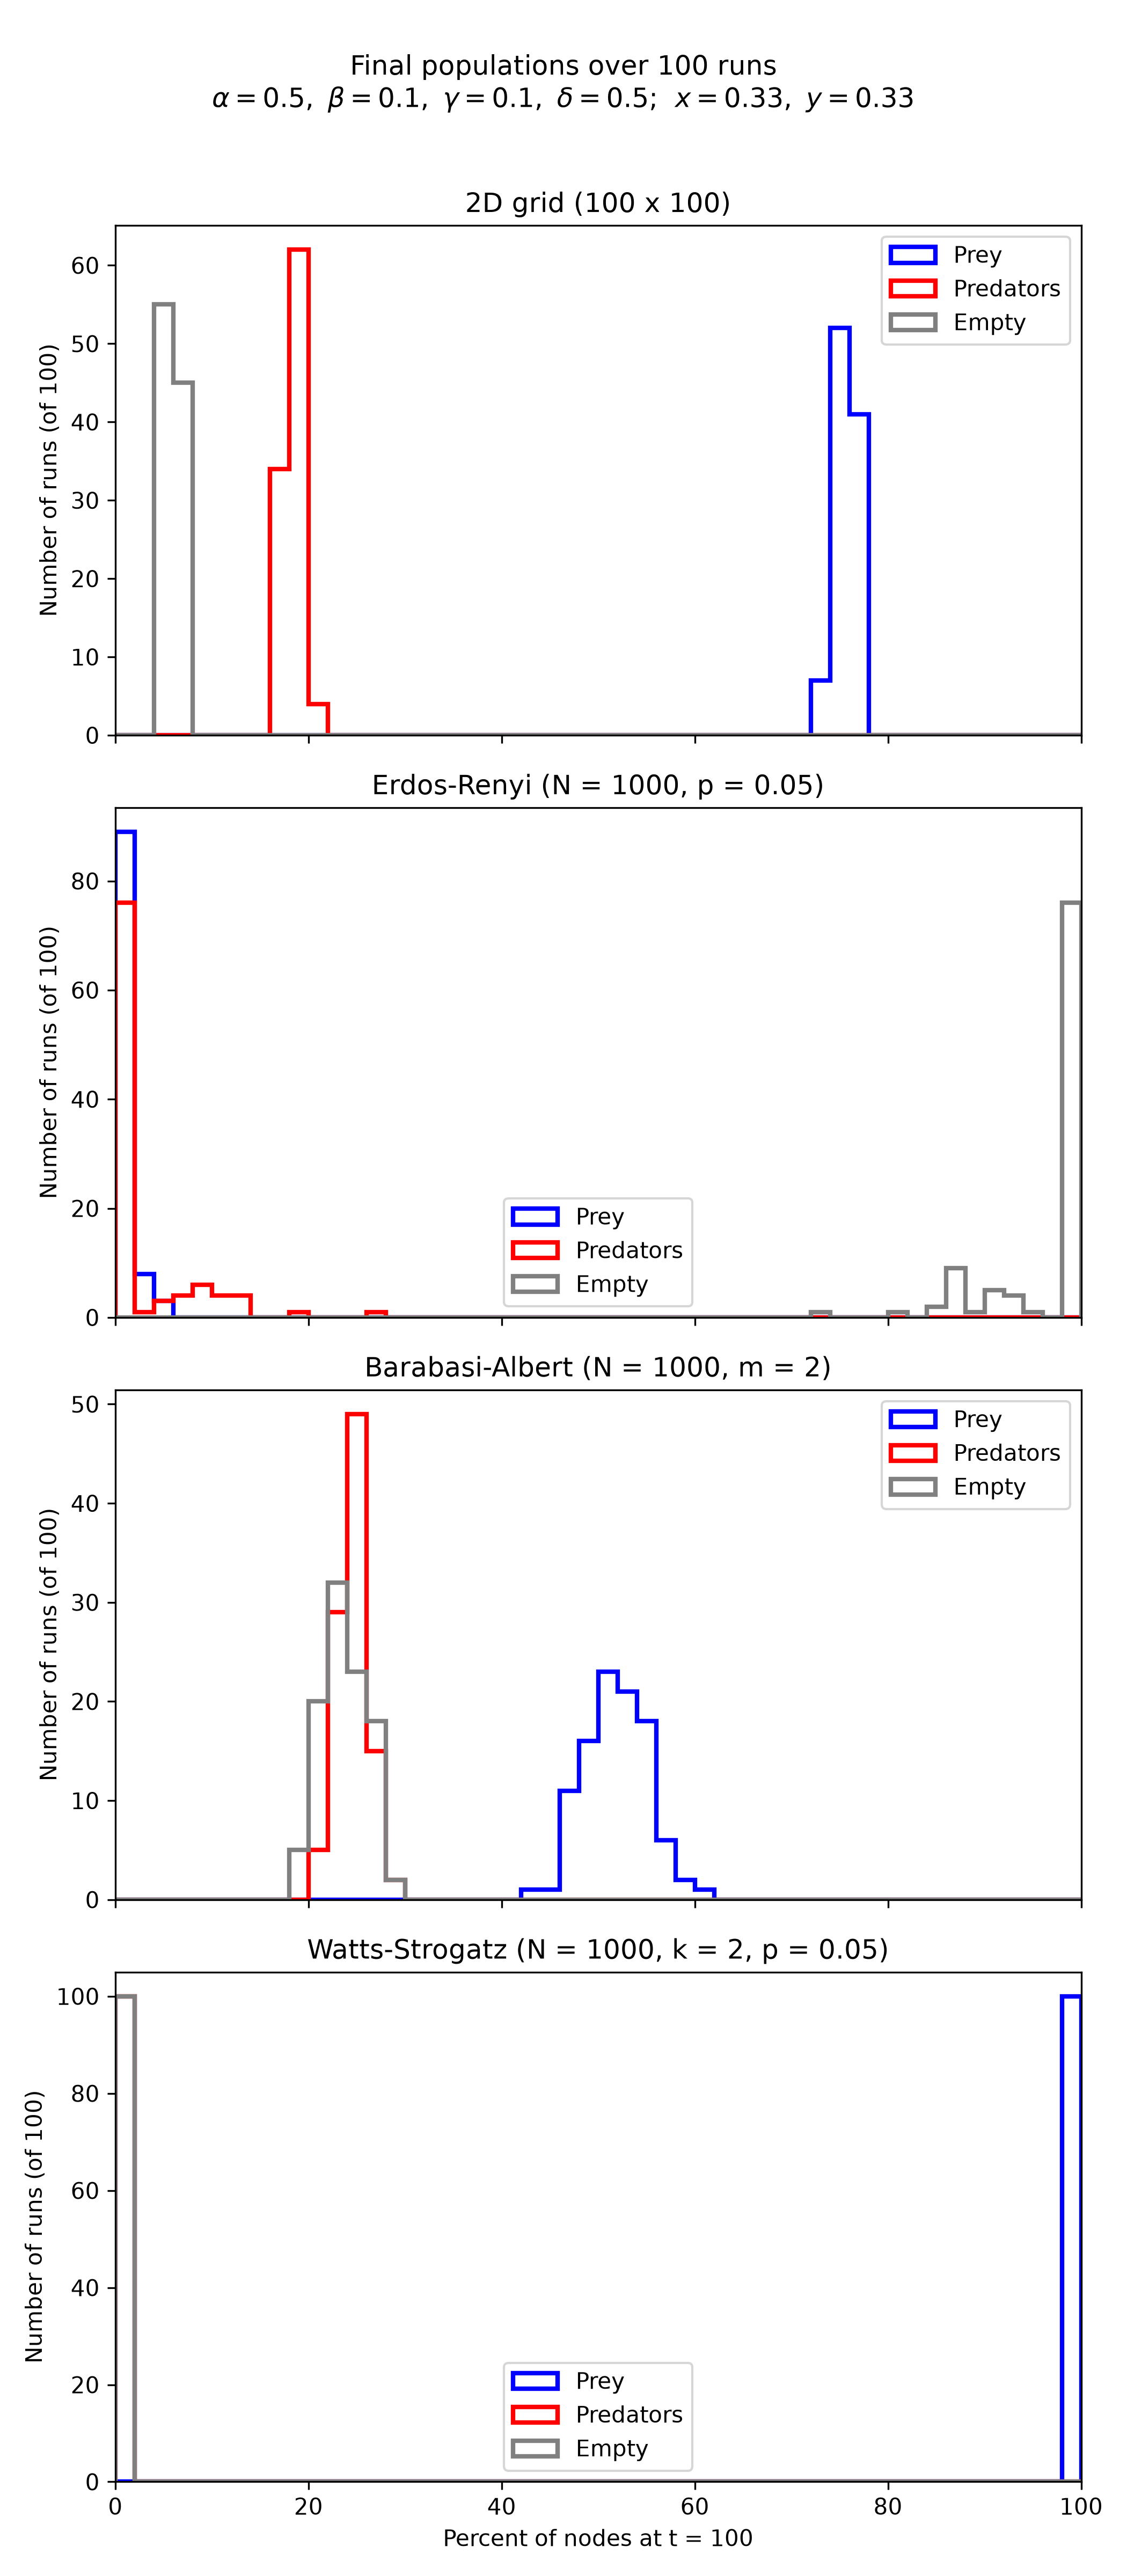
\includegraphics[height=0.85\textheight]{figures/q2b_final_histograms.png}
            \caption{Histograms of the final populations over 100 runs per graph}
            \label{q2bHistograms}
        \end{figure}

        \item In this model everything happens between direct neighbors: predators only eat prey right next to
        them, and prey only grow into empty neighbors. So what matters is how many neighbors a node has (its degree)
        and whether the structure leaves prey any refuges. Short path lengths do not really matter here, since
        nothing travels beyond one step.

        Some light math helps. A predator whose $k$ neighbors are all prey makes about $\delta\beta k$ new
        predators per step, and it dies with probability $\gamma$, so even in the best case predators can only grow if
        \begin{align*}
            \delta \beta k > \gamma \quad \Rightarrow \quad k > \dfrac{\gamma}{\delta\beta} = \dfrac{0.1}{0.5 \cdot 0.1} = 2.
        \end{align*}
        More generally, if a fraction $p$ of the nodes are prey, a typical predator sees about $p\langle k \rangle$
        prey, and the predators break even at
        \begin{align*}
            p^* = \dfrac{\gamma}{\delta\beta\langle k \rangle},
        \end{align*}
        which is the network version of the $\dfrac{\gamma}{\delta}$ prey level from 1.b. \autoref{q2cMeanField}
        compares this rough estimate to what we saw. It treats every node as having the average degree, so it ignores
        the structure, and where it fails tells us something.
        \begin{table}[ht!]
            \centering
            \begin{tabular}{lccc}
                \toprule
                Graph & $\langle k \rangle$ & $p^* = \dfrac{\gamma}{\delta\beta\langle k \rangle}$ & Mean final prey (100 runs) \\
                \midrule
                2D grid & $\approx 4$ (4 neighbors per interior node) & 50\% & 75.7\% \\
                Erd\H{o}s-R\'enyi & $p\pl N-1 \pr \approx 50$ & 4\% & 0.5\% \\
                Barab\'asi-Albert & $2m = 4$ & 50\% & 51.8\% \\
                Watts-Strogatz & $k = 2$ & 100\% & 99.7\% \\
                \bottomrule
            \end{tabular}
            \caption{Rough mean-field prey level vs. the simulations, with $\langle k \rangle$ from the graph parameters}
            \label{q2cMeanField}
        \end{table}
        \begin{itemize}
            \item \textbf{Erd\H{o}s-R\'enyi:} the high degree is what kills everything. With $\langle k \rangle \approx p\pl N-1 \pr \approx 50$,
            a typical prey starts with about $0.33 \cdot 50 \approx 16$ predator neighbors, so it is eaten with
            probability $1 - 0.9^{16} \approx 0.81$ every step. The prey are wiped out in a few steps and then the
            predators starve. ER helps the predators in the short term, but they overeat their food supply. Since
            the edges are placed at random, there is little local structure and no refuges, so it acts most like the well-mixed model,
            with a huge predation rate. Even the estimate only allows 4\% prey, and a population that small is easily
            wiped out by chance.
            \item \textbf{Watts-Strogatz:} with $k = 2$ this graph is basically a ring, where each node is only
            connected to the node on either side. A ring has no triangles, so there is (almost) no clustering, and it
            is not clustering that hurts the predators. It is the degree. Even a predator with prey on both sides only makes
            $2\delta\beta = 0.1$ new predators per step, exactly its death rate $\gamma = 0.1$, so at best the
            predators break even, and in practice they lose. The prey then fill the whole ring. WS favors the prey.
            \item \textbf{2D grid:} with degree 4 the predators can grow, but they can only ever reach 4 nodes. They
            eat out their own neighborhood and then go hungry, while the prey quickly regrow into the gaps
            ($\alpha = 0.5$). Prey in the middle of a big blue patch in \autoref{q2bGridSnapshots} have no predator
            neighbors at all, so they cannot be eaten. These patches are refuges that the estimate ignores, which is why
            the prey end at about 76\% instead of 50\%. The grid favors the prey and gives the most stable
            equilibrium, with the smallest spread across runs (SD under 1\%).
            \item \textbf{Barab\'asi-Albert:} the same average degree as the grid, but very uneven: a few hubs have
            many neighbors, while most nodes have only a few (at least $m = 2$). The hubs are surrounded by prey and become predator strongholds (the
            red top rows in \autoref{q2bArraySnapshots}), while the many low-degree nodes are rarely next to a
            predator and act as refuges for the prey. The result is the most balanced coexistence, close to the
            estimate (52\% vs. 50\%, which may be partly luck), but with the most run-to-run variation.
        \end{itemize}
        Overall, the topology mainly matters through degree (how much food each predator can reach) and structure
        (whether the prey have refuges). Too high a degree (ER) and the predators overeat and everything dies, too low
        (WS) and the predators starve and the prey win, and in between (grid, BA) the two species coexist. Unlike the
        ODE in Question 1, the network also has a built-in carrying capacity (prey can never exceed $N$) and
        extinction is permanent, so instead of neutral cycles we see the populations settle or die out. These
        conclusions are for one set of rates with $\beta$ fixed across graphs. Scaling $\beta$ by $\langle k \rangle$
        would be a natural next step to separate the effect of degree from the rest of the structure.
        \clearpage
    \end{enumerate}
\end{enumerate}
\end{solution}

\begin{problem}{5 \textbf{OPTIONAL} (5 bonus points)}
    We are nearing the end of the course. What topics do you wish we had covered, what topics do you wish we had gone into more detail on, and would you have preferred we spent less time on any topic? This will help calibrate future versions of this course, but may also influence what we cover in CNET~5052.
\end{problem}

\begin{solution}
    Your (optional) solution here...
\end{solution}

\end{document}